\documentclass[lang=cn, zihao=4.5]{elegantbook}
\usepackage{hyperref}
\usepackage{booktabs}

% font settings
\definecolor{mgreen}{RGB}{0,166,82}

% watermark settings
%\usepackage{ctex, draftwatermark, everypage}
%	\SetWatermarkText{DEEP Team 讲义模版}
%	\SetWatermarkLightness{0.95}
%	\SetWatermarkScale{0.3}

% customised commands
\newcommand{\xl}[1]{\overrightarrow{#1}}
\newcommand{\nd}[1]{〔#1〕}
\newcommand{\ssb}[1]{\left( #1 \right)}
\newcommand{\R}{\mathbb{R}}
\newcommand{\C}{\mathbb{C}}
\newcommand{\F}{\mathbb{F}}
\newcommand{\sw}[1]{\boxed{\text{解法 #1}} \ }
\newcommand{\buzhou}[1]{$#1^{\circ} \ $}
\usepackage{ulem}
	\newcommand{\tk}{\uline{\hspace{4em}}}
\newcommand{\pspace}{\vspace{0.5em}}
\usepackage{amsmath,amsfonts}
	\DeclareMathOperator{\spn}{span}
	\DeclareMathOperator{\ic}{i}
	\DeclareMathOperator{\card}{card}
	\DeclareMathOperator{\arccot}{arccot}
	\DeclareMathOperator{\setjianfa}{\textbackslash}
\newcommand{\examplefont}[1]{\color{mgreen} \textbf{#1}}

% cover settings

\title{高中数学}

\author{Johnny Tang}
\institute{DEEP Team}
\date{January 21, 2023}

\extrainfo{请:相信时间的力量,敬畏概率的准则}


\cover{cover.png}

% 本文档命令


% 修改标题页的橙色带
% \definecolor{customcolor}{RGB}{32,178,170}
% \colorlet{coverlinecolor}{customcolor}


\begin{document}

\maketitle

\frontmatter

\mainmatter

\tableofcontents

注:初等数论部分在我学完后开始编写.

\newpage

\part{预备知识}

\setcounter{chapter}{-1}
\chapter{数理逻辑与集合}

\section{数理逻辑}

\subsection{命题的概念}

\begin{definition}{命题}
	由一个陈述句表达的、具有真值的判断称为\textbf{命题}.
\end{definition}
\begin{remark}
	有一种特殊的命题,形如“若$p$,则$q$”,这种命题可以帮助我们判断很多要素.
\end{remark}

命题之间有一些特殊关系.

\begin{definition}{充分条件与必要条件} %ayumu数分p1定义0.1
	设命题$A$和$B$.若$A$可以推得$B$,则称命题$A$是$B$的\textbf{充分条件}(sufficient condition),$B$是$A$的\textbf{必要条件}(necessary condition),记作$$A \Rightarrow B,~\text{或}~B \Leftarrow A$$
	若$A$可以推得$B$且$B$可以推得$A$,则称命题$A$和$B$互为\textbf{充分必要条件}(necessary and sufficient condition),简称充要条件,此时也称命题$A$和$B$等价($A$成立当且仅当$B$成立),记作$$A \Leftrightarrow B$$
	此时$B \Rightarrow A$的过程称为充分性,$A \Rightarrow B$的过程称为必要性.
\end{definition}
\begin{remark}
	还有一个类似的逻辑语言:有且仅有(恰有),这意味着存在一个(存在性)且只有一个(唯一性).例如,平面中,过直线外一点有且仅有一条直线与之平行.
\end{remark}

可以用图像来更好理解该定义.

\begin{figure}[h!]
	\centering
	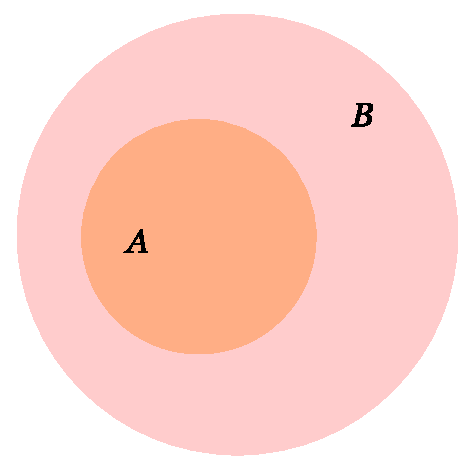
\includegraphics[width=5cm]{attachment/202302191.pdf}
	\caption{例如,此时$A$是$B$的必要且不充分条件}
\end{figure}

\begin{example}
	(1)一个四边形“是菱形”是“它的对角线互相垂直”的\tk 条件. \\
	(2)“$0<x<1$”是“$x<2$”的\tk 条件. \\
	(3)设有命题$p,q$.则“$p \Rightarrow q$”是“$p \Leftrightarrow q$”的\tk 条件. \\
	(4)“$x^2-5x+6 \neq 0$”是“$x \neq 2$”的\tk 条件.
\end{example}
\begin{solution}
	(1)充分且不必要;(2)充分且不必要;(3)必要且不充分;(4)必要且不充分.
\end{solution}

不过这种直观的判断方式比较迷惑,我们可以通过命题的逻辑运算更好地思考这些问题.

\begin{definition}{命题的逻辑运算} %ayumu数分p1定义0.3
	设命题$A$与$B$, \\
	(1)若$A$和$B$中至少有一个命题成立,则称$A$\textbf{或}(or)$B$,记作$$A \vee B$$
	(2)若$A$和$B$同时成立,则称$A$\textbf{且}(and)$B$,记作$$A \wedge B$$
	(3)若$A$的相反形式成立,则称\textbf{非}(not)$A$(或称$A$的否定),记作$$\neg A$$
\end{definition}
\begin{remark}
	关于“且”“或”的否定,存在如下规律:
	$$\neg (A \vee B) = (\neg A) \wedge (\neg B)$$
	$$\neg (A \wedge B) = (\neg A) \vee (\neg B)$$
\end{remark}

另外,对于任意命题的否定,有一个重要法则.在二值逻辑中,该定律实际上告诉我们一个命题$P$要么为真、要么为假.

\begin{proposition}{排中律}
	对于任何命题$P$,$P \vee (\neg P)$为真.
\end{proposition}

\begin{definition}{存在,任意}
	设命题$A$, \\
	(1)若\textbf{存在}(exist)$x$使得命题$A$成立,可以记作$$\exists x~s.t.~A$$
	(2)若对于\textbf{任意}(for all)$x$都能使得命题$A$成立,可以记作$$\forall x,A$$
\end{definition}
\begin{remark}
	“$s.t.$”是“\textit{such that}”的缩写.
\end{remark}
\begin{remark}
	“存在”与“任意”的否定如下:
	$$\neg (\forall x,A) = \exists x~s.t.~\neg A$$
	$$\neg (\exists x~s.t.~A) = \forall x,\neg A$$
\end{remark}

\subsection{特殊的命题}

我们可以对特殊的“若$p$,则$q$”型命题进行更进一步的讨论.

\begin{definition}{原命题,逆命题,否命题,逆否命题}
	设有\textbf{原命题}(primitive proposition)可以表示为$P \Rightarrow Q$的形式. \\
	(1)\textbf{逆命题}(converse proposition)定义为:$$Q \Rightarrow P$$
	(2)\textbf{否命题}(inverse proposition)定义为:$$\neg P \Rightarrow \neg Q$$
	(3)\textbf{逆否命题}(contrapositive proposition)定义为:$$\neg Q \Rightarrow \neg P$$
\end{definition}
\begin{remark}
	此时否命题就是原命题的否定形式,即$\neg (P \Rightarrow Q) = (\neg Q \Rightarrow \neg P)$.
\end{remark}

回顾上一个例题的最后一问,除了用直观的判断方式以外,我们还可以用反证法说明“若$x \neq 2$,则$x^2-5x+6 \neq 0$”.实际上,反证法的本质就是以下命题所述:

\begin{proposition}
	逆否命题与原命题的真假性相同.
\end{proposition}

这个命题也可用图像来解释:

\begin{figure}[h!]
	\centering
	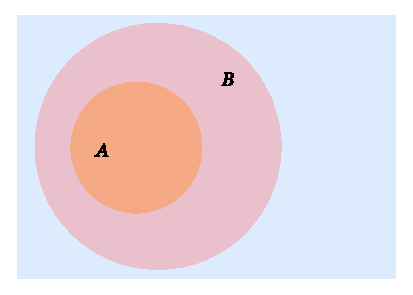
\includegraphics{attachment/202302192.pdf}
	\caption{逆否命题与原命题的真假性比较}
\end{figure}

容易发现,其中“若$A$,则$B$”就等价于“若$\neg B$(即矩形除去大圆的区域),则$\neg A$(即矩形除去小圆的区域)”.




\begin{example}
	证明:$\sqrt{2}$是无理数.
\end{example}
\begin{proof}
	设原命题:“所有能表示为$\dfrac{p}{q}~$($p,q$都是正整数且互质)的形式的数都是有理数”$\Rightarrow$“$\sqrt{2}$是无理数”. \\
	则原命题等价于“所有不能表示为$\dfrac{p}{q}~$($p,q$都是正整数且互质)的形式的数都是无理数”$\Rightarrow$“$\sqrt{2}$是无理数”. \\
	构造逆否命题:“$\sqrt{2}$是有理数”$\Rightarrow$“存在一个不能表示为$\dfrac{p}{q}~$($p,q$都是正整数且互质)的形式的数是有理数”, \\
	由“$\sqrt{2}$是有理数”,假设$\sqrt{2}= \dfrac{p}{q}~$($p,q$都是正整数且互质).两边同时平方,有$$2q^2=p^2$$
	这要求$p$是$2$的倍数,因而$p^2$是$4$的倍数,故$q^2$是$2$的倍数.又因为$q$是整数,所以$q$是$2$的倍数,那么$p,q$不互质,即$\sqrt{2}$不能表示为上述形式.这就证明了“存在一个不能表示为$\dfrac{p}{q}~$($p,q$都是正整数且互质)的形式的数是有理数”.由于原命题与逆否命题的真假性相同,故原命题也成立.
\end{proof}

\newpage
\section{集合}

\subsection{集合的概念}

一般地,把一些能够确定的不同的对象看成一个整体,就说这个整体是由这些对象的全体构成的\textbf{集合}(set).其中,构成集合的每一个对象称为\textbf{元素}(element).集合中的元素满足如下性质:确定性,互异性,无序性.特别地,一个集合可以没有元素,这样的集合叫做空集,记作$\varnothing$.

若$x$是集合$X$中的元素,则称$x$\textbf{属于}(belongs to)$X$,记作$x \in X$.反之,$x$\textbf{不属于}$X$记作$x \notin X$.

对于一个集合,我们有两种方式描述集合中的元素:

(1)列举法:将集合中的元素一一列举,例如$$\{ 1,2,3,\cdots \}$$其中“$\cdots$”表示类似的元素.

(2)描述法:为了描述含有无限个元素的集合(即无限集),我们用所含元素的性质来表示该集合,例如$$\kaishu \{ x \in E|P(x) \},~\text{或}\{ x \in E:P(x) \}$$\songti 其中$x$为这些元素的代表元素,$E$是$x$的范围,$P(x)$表示$x$满足的性质.

另外,一些常见的数集有它们特定的表示符号:

\begin{table}[h]
	\centering
	\renewcommand\arraystretch{1.3}
	\begin{tabular}{cc}
		\toprule
		符号           & 数集                    \\
		\midrule
		$\R$         & 实数(real number)集      \\
		$\mathbb{Q}$ & 有理数(rational number)集 \\
		$\mathbb{Z}$ & 整数(integer)集          \\
		$\mathbb{N}$ & 有理数(natural number)集 \\
		\bottomrule
	\end{tabular}
\end{table}

为了描述类似于“正整数集”的集合,我们规定一些标记.例如,$\R ^{+}$(或$\R _{+}$)表示正实数集,$\mathbb{Z}^{-}$表示负整数集,$\mathbb{N}^{*}$表示正有理数集(等价于正整数集).

\begin{example}
	(1)集合$A=\{ 2,0,1,3 \},~B = \{ x|-x \in A,2-x^2 \notin A \}$,则集合$B$中所有元素的和为\tk . \\
	(2)由三个实数构成的集合,既能表示为$\{ a,1,b/a \}$,也能表示为$\{ a^2,a+b,0 \}$,则$a^{99}+b^{99}=$\tk . \\
	(3)给定实数集合$A,B$,定义运算$A \oplus B = \{ x|x=ab+a+b,a \in A,b \in B \}$.设$A = \{ 0,2,4,\cdots ,18 \},~B= \{ 98,99,100 \}$,则$A \oplus B$中所有元素之和为\tk .
\end{example}
\begin{solution}
	% TODO 例题待解答
\end{solution}

以下介绍集合之间的关系:

\begin{definition}{子集和母集}
	设集合$A$和$B$,若$$\forall x,~x \in A \Rightarrow x \in B$$则称$A$\textbf{包含于}(is included in)$B$,或$B$\textbf{包含}(includes)$A$;$A$是$B$的一个\textbf{子集}(subset),$B$是$A$的一个\textbf{母集}(superset),记作$$A \subseteq B,~ \text{或} B \supseteq A$$
	
	当$A$和$B$互为子集时,记作$A=B$.即,$A=B$表示$$\forall x,~ x \in A \Leftrightarrow x \in B$$
	
	特别地,若$$(A \subseteq B) \wedge (A \neq B)$$则称$A$是$B$的一个\textbf{真子集}(proper subset),$B$是$A$的一个\textbf{真母集}(proper superset),记作$$A \subsetneqq B,~ \text{或} B \supsetneqq A$$
\end{definition}
\begin{note}
	上述定义中符号“$\subseteq ,\subsetneqq$”在一些数学课本中也会写作“$\subset$”等.本书均采用上述写法.
\end{note}

由上述定义,不难证明,空集是任意集合的子集、是任意非空集合的真子集.

有时我们需要研究某个有限集合的元素个数.设有限集$A$,可以用$\card (A)$表示其元素个数(card即\textit{cardinal},基数).另外,有限集$A$的\textbf{阶}也表示其元素个数,记作$|A|$.

\begin{example}
	证明:对于一个有限集$A$,它的子集个数为$2^{|A|}$个,真子集个数为$2^{|A|}-1$个.
\end{example}
\begin{solution}
	% TODO 例题待解答
\end{solution}
\begin{example}
	设$\{ b_n \}$是集合$\{ 2^t+2^s+2^r | 0 \leq r < s < t,~r,s,t \in \mathbb{Z} \}$中所有的数从小到大排列成的数列,已知$b_k=1160$,求$k$.
\end{example}
\begin{solution}
	% TODO 例题待解答
\end{solution}

\subsection{集合间的运算与运算律}

类似于上文对子集和母集的定义,我们可以从集合中元素的角度来研究集合间的运算.

\begin{definition}{集合的交、并、差、补}
	设集合$A$和$B$, \\
	(1)$A$与$B$的\textbf{交集}(intersection),记作$A \cap B$,定义为$$A \cap B = \{ x|(x \in A) \wedge (x \in B) \}$$
	(2)$A$与$B$的\textbf{并集}(union),记作$A \cup B$,定义为$$A \cup B = \{ x|(x \in A) \vee (x \in B) \}$$
	(3)$A$与$B$的\textbf{差集}(difference),记作$A-B$或$A \setjianfa B$,定义为$$A \setjianfa B = \{ x|(x \in A) \wedge (x \notin B) \}$$
	(4)设$U$为\textbf{全集}.$A$的\textbf{补集}(complement),记作$\complement _{U}{A}$,定义为$$\complement _{U}{A} = \{ x|(x \in U) \wedge (x \notin A) \}$$
	若已知该全集(题目中明确定义),$A$的补集也可记作$\overline{A}$.
\end{definition}

就像对于加减乘除运算,我们要研究其运算律一样,集合的交、并、补运算也有类似的运算律.

\begin{proposition}{集合运算的运算律}
	设集合$A$和$B$,全集$U$. \\
	(1)它们的交、并运算满足交换律,即$$A \cap B = B \cap A \qquad A \cup B = B \cup A$$
	(2)它们的交、并运算满足结合律,即
	$$A \cap B \cap C = (A \cap B) \cap C = A \cap (B \cap C)$$
	$$A \cup B \cup C = (A \cup B) \cup C = A \cup (B \cup C)$$
	(3)它们的交运算与并运算之间满足分配律,即
	$$(A \cap B) \cup C = (A \cup C) \cap (B \cup C)$$
	$$(A \cup B) \cap C = (A \cap C) \cup (B \cap C)$$
	(4)它们的交、并运算与补运算之间满足摩根律(或称德摩根定理,De Morgan's theorem),即$$\overline{A \cap B} = \overline{A} \cup \overline{B} \qquad \overline{A \cup B} = \overline{A} \cap \overline{B}$$
\end{proposition}

\begin{example}
	(1)已知$A=\{ 2,5 \}$,$B = \{ x|x^2+px+q=0 \}$,且$A \cup B = A$,$A \cap B = \{ 5 \}$,则$pq=$\tk . \\
	(2)已知$M,N$均为$\mathbb{R}$的子集,且$(\complement _{\mathbb{R}} M) \subseteq N$,则$M \cup (\complement _{\mathbb{R}} N)=$\tk . \\
	(3)设集合$A = \{ x|1 \leq x \leq 2000,~x \in \mathbb{N} \}$,$B = \{ x|1993 \leq x \leq 2021,~x \in \mathbb{N} \}$.则满足$S \subseteq A$,且$S \cap B \neq \varnothing$的集合$S$的个数为\tk .
\end{example}
\begin{solution}
	% TODO 例题待解答
\end{solution}

实际上,集合之间的交、并与逻辑运算中的和、或是一样的.例如,不等式$x^2-4x+3 \geq 0$的取值范围为$$\{ x|(x \leq 1) \vee (x \geq 3) \} = \{ x|x \leq 1 \} \cup \{ x|x \geq 3 \}$$

为了更方便地表示上述结果,引入区间的概念:

\begin{definition}{区间}
	定义$\R$上的一种特殊数集为\textbf{区间}(interval).例如 \\
	$$(a,b):=\{ x \in \R | a<x<b \} \quad \textit{“开区间”}$$
	$$[a,b]:=\{ x \in \R | a \leq x \leq b \} \quad \textit{“闭区间”}$$
	$$(a,b]:=\{ x \in \R | a<x \leq b \} \quad \textit{“左开右闭区间”}$$
	$$(-\infty,b):=\{ x \in \R | x<b \}$$
	$$[a,+\infty):=\{ x \in \R | x \geq a \}$$
	$$(-\infty ,+\infty):= \R $$
	其他形式的区间定义相似.
\end{definition}

上文例子中$x$的取值范围就可以表达为$$(-\infty ,1] \cup [3,+\infty )$$


\chapter{对数运算}

在介绍对数运算之前,我们需要了解\textbf{幂}(power)的概念.对于单项式$a^n(n \in \mathbb{Q})$,令$n=\frac{p}{q}$,
$$a^{\frac{p}{q}}:=\sqrt[q]{a^p} \ (p,q \in \mathbb{Z})$$

这就是有理数次幂的严格定义.其中,$a$称为底数,$n$称为指数,$a^n$的值称为幂值.若$n$是无理数,可以通过计算有理数次幂进行逼近计算.

在初中我们常常遇到一类问题:例如,求$2$的多少次方是$1024$.这种简单的式子还可以一眼看出结果,那么$2$的多少次方是$1023$呢?这就不好说明.更进一步,我们甚至找不到一个比较好的逼近计算的方式.于是人们发明了对数运算:

一般地,若$a^x=y~(a>0,a \neq 1)$,则称$x$为以$a$为底$y$的\textbf{对数}(logarithm),记作$x = \log_{a}{y}$,其中$a$叫做底数,$y$叫做真数.通常把以$10$为底的对数叫做\textbf{常用对数}(common logarithm)(化学中pH值的计算公式就包括它),简记为$\log_{10}{N}=\lg N$;把以自然常数$e$为底的对数叫做\textbf{自然对数},简记为$\log_{e}{N}=\ln N$.

对数运算有两条重要性质:(1)$~\log_{a}{1} = 0,~\log_{a}{a}=1$;(2)$~a^{\log_{a}{N}}=N$.第二条看起来是个废话,其实很有用.

\begin{example}
	计算:$\log_{2}{8}=$\tk ,~$\log_{\sqrt{5}}{125}=$\tk ,~$\log_{114514}{1}=$\tk ,$\log_{8}{16}=$\tk .
\end{example}

类似于指数运算,对数运算也有一些重要运算公式:

\begin{proposition}{对数的运算法则}
	假设下列式子都有意义. \\
	(1)加减法$$\log_{\alpha}{MN} = \log_{\alpha}{M} + \log_{\alpha}{N} \qquad \log_{\alpha}{\frac{M}{N}} = \log_{\alpha}{M} - \log_{\alpha}{N}$$
	(2)换底公式$$\log_{\alpha}{x} = \frac{\log_{\beta}{x}}{\log_{\beta}{\alpha}}$$
	(3)指数$$\log_{\alpha ^n}{x^m} = \frac{m}{n} \log_{\alpha}{x}$$
	(4)倒数$$\log_{\alpha}{\beta} = \frac{1}{\log_{\beta}{\alpha}}$$
	(5)链式$$\log_{\alpha}{\beta} \cdot \log_{\beta}{\gamma} = \log_{\alpha}{\gamma}$$
\end{proposition}
\begin{proof}
	这里只选择部分运算法则证明: \\
	(1)加法:由对数的定义,$\alpha ^{\log_{\alpha}{M}} = M,~\alpha ^{\log_{\alpha}{N}} = N$,于是$$MN = \alpha ^{\log_{\alpha}{M}} \cdot \alpha ^{\log_{\alpha}{N}} = \alpha ^{\log_{\alpha}{M} + \log_{\alpha}{N}}$$
	这告诉我们$\log_{\alpha}{MN} = \log_{\alpha}{M} + \log_{\alpha}{N}$. \\
	(2)换底公式:由对数的定义,$\beta ^{\log_{\beta}{x}} = x,~\beta ^{\log_{\beta}{\alpha}} = \alpha$,那么$$x = (\beta ^{\log_{\beta}{\alpha}})^{\frac{\log_{\beta}{x}}{\log_{\beta}{\alpha}}} = \alpha ^{\frac{\log_{\beta}{x}}{\log_{\beta}{\alpha}}}$$
	这告诉我们$\log_{\alpha}{x} = \dfrac{\log_{\beta}{x}}{\log_{\beta}{\alpha}}$. \\
	(5)链式:令$$\log_{\alpha}{\beta} = \frac{\ln{\beta}}{\ln{\alpha}},~ \log_{\beta}{\gamma} = \frac{\ln{\gamma}}{\ln{\beta}}$$
	所以$$\log_{\alpha}{\beta} \cdot \log_{\beta}{\gamma} = \frac{\ln{\beta}}{\ln{\alpha}} \cdot \frac{\ln{\gamma}}{\ln{\beta}} = \frac{\ln{\gamma}}{\ln{\alpha}} = \log_{\alpha}{\gamma}$$
\end{proof}
\begin{remark}
	不难发现,在应用换底公式之后做证明变得很轻松.可以说,如果把“重要性质”比作一个轮子,那么换底公式就是一辆车:用轮子也能向前走(用重要性质也能写证明),但远不及一辆车快速与舒适(引入换底公式会十分便捷).
\end{remark}
\begin{remark}
	换底公式的本质是找到了一个“工具对数”作为中间量化简计算,就跟我们倾向于使用$\dfrac{1}{7}$而不是$0.142857\cdots$一样.
\end{remark}
\begin{remark}
	由加减法运算法则,可以一窥常用对数的作用.例如,
	$$\lg{120} = \lg{1.2 \times 10^2} = \lg{1.2}+2$$
	$$\lg{0.012} = \lg{1.2 \times 10^{-2}} = \lg{1.2}-2$$
	若要计算$\lg{120}$与$\lg{0.012}$,只需要知道$\lg{1.2}$的值.于是$\lg{N}$可以被用在换底公式中作为“工具对数”来近似计算.
\end{remark}

\chapter{多项式与代数变换}

\section{多项式与Vieta定理}

多项式,多项式间的关系与运算,多项式的带余除法,多项式的根,余数定理,因式定理,Vieta定理

\begin{definition}{多项式}
	形如$$f(x) = a_nx^n + \cdots + a_1x + a_0~(a_n \neq 0)$$的表达式称为关于$x$的一元$n$次\textbf{多项式}(polynomial),其中$n$称为多项式的\textbf{次数},记作$\deg f = n$.规定恒等于$0$的多项式的次数为$-\infty$.
\end{definition}

\begin{definition}{多项式间的关系与运算}
	设$f(x) = \sum_{k=0}^{n}a_kx^k,~g(x) = \sum_{k=0}^{m}b_kx^k$.不妨设$n \geq m$,规定$b_k=0~(k > m)$.
	\begin{itemize}
		\item $f(x)=g(x)$的充要条件是$n=m,~a_k=b_k$.
		\item 多项式的加减法定义如下:$$f(x) \pm g(x) := \sum_{k=0}^{n} (a_k \pm b_k)x^{k}$$
		\item 多项式的乘法定义如下:$$f(x) \cdot g(x) := \sum_{k=0}^{m+n} \ssb{\sum_{i+j=k}a_ib_j}x^k$$
	\end{itemize}
\end{definition}

\begin{proposition}{多项式的带余除法}
	若$f(x)$和$g(x)$是两个已知的多项式,其中$g(x)$不是零多项式,那么存在唯一的一对多项式$q(x)$和$r(x)$,使得$$f(x) = g(x) \cdot q(x) + r(x)$$其中$\deg r < \deg g$或$r(x)=0$.称$q(x)$和$r(x)$分别为$f(x)$除以$g(x)$所得的\textbf{商式}与\textbf{余式}.
\end{proposition}

\section{整式恒等变形}

换元技巧,齐次性原理

\section{简单的不等式}

绝对值不等式,糖水不等式,均值不等式,线性规划

\part{函数与数列}

\chapter{函数}

\section{映射与函数}

\subsection{映射与函数的概念}

\begin{definition}{映射}
	\begin{itemize}
		\item 设$A$和$B$为两个集合,若对$A$中每个元素$x$,都存在$B$中唯一的元素$y$与之对应,则称此对应关系为一个\textbf{映射}(map),记作$$f:A \to B,~~x \mapsto y$$
		\item $x$在$B$中的对应元素$y$称为$x$在$f$下的\textbf{象}(image),$x$称为$y$在$f$下的\textbf{原象}(preimage),记作$$f(x) = y,~ x \in A$$
		\item 集合$A$称作映射$f$的\textbf{定义域}(domain),记作$D_f$;集合$B$称为映射$f$的\textbf{陪域}(codomain);$A$中所有元素在$f$下的象组成的集合称为$f$的\textbf{值域}(range),记作$R_f$或$f(D)$.
		\item 两个映射相等,当且仅当它们的定义域、对应关系、值域相同.
	\end{itemize}
\end{definition}

定义域、陪域与值域的关系如下:

% TODO 定义域、陪域、值域的关系作图

\begin{definition}{特殊的映射}
	设映射$f:A \to B$.
	\begin{itemize}
		\item 若$A$中的每一个$x$的唯一对应$B$中的一个$f(x)$,则称$f$是\textbf{单射}(injection).
		\item 若对于$B$中的每一个元素$y$,总能找到$A$中的一个$x$使得$f(x)=y$,则称$f$是\textbf{满射}(surjection).
		\item 若$f$既是单射,又是满射,则称$f$是\textbf{双射}(bijection).
	\end{itemize}
\end{definition}

单射、满射、双射举例如下:

% TODO 单射、满射、双射举例作图

\subsection{映射与函数的运算}

先介绍一种由定义自然产生的运算:

\begin{definition}{逆映射与反函数} %兴趣一阶I p26
    设映射$f:A \to B$,如果$f$是一个双射,则对任意的$y \in B$,都存在唯一的$x \in A$使得$y=f(x)$.这就产生了一个从$B$到$A$的映射,称为$f$的\textbf{逆映射}(inverse mapping),记作$$f^{-1}:B \to A$$
    对于这样的逆映射,它的定义域是$B$,值域是$A$.\\
    同样地,设函数$f:A \mapsto B$,如果$f$是一个双射,则$f$的逆映射$f^{-1}$称为函数$f$的\textbf{反函数}(inverse function),其定义域是$B$,值域是$A$.
\end{definition}

不难发现,如果两个函数互为反函数,它们的图像关于$y=x$对称.

函数间加减法的定义很符合直觉.

\begin{definition}{函数的加减法}
	对于$f,g:A \to B$,对所有$x \in A$,规定函数的加减法$f \pm g$满足$$(f \pm g)(x) = f(x) \pm g(x)$$
	函数$f \pm g$的定义域为$A$,陪域不定.
\end{definition}

那么函数之间的乘法该是如何的?实际上,如果单纯地将$f(x)$与$g(x)$的值相乘,得到的新函数很难研究.我们更倾向于研究一种特殊的“乘法”:

\begin{definition}{映射与函数的复合} %兴趣一阶I p26
    设映射$f:A \to B$,$g:B \to C$,则它们的\textbf{复合映射}(composite mapping)$gf:A \to C$定义为$$(gf)(x)=g(f(x)) \ (x \in A)$$
    注意复合运算有先后顺序.容易说明映射$gf$的定义域为$A$,值域为$C$.\\
    当集合$A,B,C$均为数集时,可以得到类似的复合函数定义.
\end{definition}
\begin{remark}
	为了强调复合运算,$gf$也可记作$g \circ f$.
\end{remark}

\section{常见初等函数}

初等函数,是指用基本初等函数进行有限次加减乘除、乘方、开方、复合操作后得到的函数.

在中学阶段可以遇见的基本初等函数,大致可以分为以下几类:常值函数、指数函数、对数函数、幂函数、三角函数、反三角函数.对于这些函数的概念、图像与性质,我们逐一介绍.(注:三角函数与反三角函数在下一章介绍)

\subsection{基本初等函数}

\begin{definition}{常值函数}
    形如$$f(x)=C \ (C \in \mathbb{R}, C\textit{是常数})$$
    的函数称为\textbf{常值函数}(constant function).它的定义域为$\mathbb{R}$,值域为${C}$.
\end{definition}

\begin{definition}{幂函数}
    形如$$f(x)=x^{\alpha} \ (\alpha \text{是常数})$$
    的函数称为\textbf{幂函数}(power function).
\end{definition}

幂函数的性质不过多介绍.只需知道例如$f(x)=x^3$或$f(x)=\sqrt[4]{x}$的函数都是幂函数.

\begin{definition}{指数函数}
    形如$$f(x)=a^x, \ a>0 , a\neq 1$$
    的函数称为\textbf{指数函数}(exponential function).
\end{definition}

\begin{proposition}{指数函数的性质}
    指数函数$f(x)=a^x$具有以下性质:
    \begin{itemize}
        \item 定义域:$\mathbb{R}$
        \item 值域:$\mathbb{R}^+$
        \item 单调性:当$0<a<1$时,为减函数;当$a>1$时,为增函数
        \item 图像:恒过定点$(0,1)$
    \end{itemize}
\end{proposition}
\begin{remark}
    单调性参考后文:函数的性质.
\end{remark}

% TODO 指数函数的图像

\begin{definition}{对数函数}
    形如$$f(x)=\log_{a}{x}, \ a>0,a \neq 1$$
    的函数称为\textbf{对数函数}(logarithmic function).它的定义域为$\mathbb{R}^{+}$,值域为$\mathbb{R}$
\end{definition}

\begin{proposition}{对数函数的性质}
    对数函数$f(x)=\log_{a}{x}$具有以下性质:
    \begin{itemize}
        \item 定义域:$\mathbb{R}^{+}$
        \item 值域:$\mathbb{R}$
        \item 单调性:当$0<a<1$时,为减函数;当$a>1$时,为增函数
        \item 图像:恒过定点$(1,0)$
    \end{itemize}
\end{proposition}

% TODO 对数函数的图像

实际上,我们发现对数函数$f(x)=\log_{a}{x}$与指数函数$f=a^{x}$($a>0$且$a \neq 1$)互为反函数.它们的图像关于$y=x$对称.

\subsection{对勾函数与飘带函数}

有两类特殊的初等函数,在研究最值问题时很常见.

\begin{problem}
    设函数$$f(x)=mx+\frac{n}{x}~(m,n>0)$$
    请指出它的定义域、值域并作出示意图.
\end{problem}
\begin{solution}
    XXX
\end{solution}

还有一种类似于对勾函数,但没什么研究价值的函数.我们可以形象地称之为“垃圾函数”,虽然大多数人都会叫它“飘带函数”.

\begin{problem}
    设函数$$f(x)=mx-\frac{n}{x}~(m,n>0)$$
    请指出它的定义域、值域并作出示意图.
\end{problem}
\begin{solution}
    XXX
\end{solution}

\section{函数的性质}

\subsection{单调性}

先介绍单调性的概念:

\begin{definition}{函数的单调性} %兴趣一阶I p66
    设函数$f(x)$的定义域为$D$,区间$I \subseteq D$.\\
    若对任意$x_1,x_2 \in I$,且$x_1 < x_2$,有$f(x_1) < f(x_2)$,则称$f(x)$\textbf{单调递增}(monotonically increasing),也称$f(x)$为增函数.\\
    反之,若对任意$x_1,x_2 \in I$,且$x_1 < x_2$,有$f(x_1) > f(x_2)$,则称$f(x)$\textbf{单调递减}(monotonically decreasing),也称$f(x)$为减函数.\\
    如果函数$f(x)$在某个区间$I$上是增函数或减函数,那么就说函数$f(x)$在这个区间上具有\textbf{单调性}(monotonicity).区间$I$叫做$f(x)$的单调区间.
\end{definition}
\begin{remark}
    有些时候,将定义中的条件分别改为$f(x_1) \leq f(x_2)$、$f(x_1) \geq f(x_2)$的函数,也被称为不减函数、不增函数.
\end{remark}
\begin{note}
    要注意描述单调区间的语言:例如,\\
    函数$$f(x)=\frac{1}{x}$$
    在$(- \infty , 0)$\color{red}{和}\color{black}$(0 , + \infty)$上单调递减.它有两个单调区间,而不能看做一整个,这是因为存在例如$f(-1) < f(1)$的情况;\\
    函数$$ f(x)=\begin{cases}
    	x &x<0 \\
    	x+1 &x>0
    \end{cases}$$
    在$(- \infty , 0) \color{red}{\cup}\color{black} (0 , + \infty)$上单调递增.它只有一个单调区间.
\end{note}

注意到,如果一个函数在某个区间上连续且单调,它在这个区间上一定是个单射.(注:所有初等函数都是连续的)

\begin{proposition}{函数单调性的变化规律}
    设函数$f(x),g(x)$,为了方便计算,假定它们的定义域相同、单调区间相同.\\
    (1)函数的加法$f(x)+g(x)$:增函数$+$增函数 $\Rightarrow$ 增函数;减函数$+$减函数 $\Rightarrow$ 减函数.\\
    (2)函数的减法$f(x)-g(x)$:增函数$-$减函数 $\Rightarrow$ 增函数;减函数$-$增函数 $\Rightarrow$ 减函数.\\
    (3)函数的乘法、除法、乘方、开方:具体情况分析.\\
    (4)函数的复合$f(x) \circ g(x)$:增函数 $\circ$ 增函数 $\Rightarrow$ 增函数;增函数 $\circ$ 减函数 $\Rightarrow$ 减函数;减函数 $\circ$ 增函数 $\Rightarrow$ 减函数;减函数 $\circ$ 减函数 $\Rightarrow$ 增函数.
\end{proposition}
\begin{proof}
    XXX
\end{proof}

\begin{theorem}{区间根定理}
    假设函数$f(x)$满足以下条件:
    \begin{enumerate}
        \item 在区间$a \leq x \leq b$上连续;
        \item $f(a) \cdot f(b)<0$.
    \end{enumerate}
    则在区间$a<x<b$上必定存在至少一个$c$,使得$f(c)=0$.\\
    或者说,当一个函数在$x=a$时有$f(x)<0$且在$x=b$时有$f(x)>0$,那么它必然有至少一个零点$c$,其中$a<c<b$.反之亦然.
\end{theorem}

\subsection{奇偶性与对称性}

先介绍奇偶性的概念:

\begin{definition}{奇偶性} %兴趣一阶I p66
    设函数$f(x)$,其定义域$D$关于原点对称.\\
    若对任意$x \in D$,$f(x)=-f(-x)$,则称$f(x)$为\textbf{奇函数}(odd function).\\
    反之,若对任意$x \in D$,$f(x)=f(-x)$,则称$f(x)$为\textbf{偶函数}(even function).\\
    显然,奇函数的图像沿原点中心对称,偶函数的图像沿$y$轴轴对称.
\end{definition}

\begin{proposition}{函数奇偶性的变化规律}
    设函数$f(x),g(x)$,为了方便计算,假定它们的定义域相同.\\
    (1)同奇偶性函数的加减法$f(x) \pm g(x)$:奇函数$\pm$奇函数 $\Rightarrow$ 奇函数;偶函数$\pm$偶函数 $\Rightarrow$ 偶函数.\\
    (2)不同奇偶性函数的加减法:具体情况分析.\\
    (3)函数的乘法$f(x) \cdot g(x)$:奇函数$\cdot$奇函数 $\Rightarrow$ 偶函数;偶函数$\cdot$偶函数 $\Rightarrow$ 偶函数;奇函数$\cdot$偶函数 $\Rightarrow$ 奇函数.\\
    (4)函数的除法:$\frac{1}{\text{奇函数}}$ $\Rightarrow$ 奇函数;$\frac{1}{\text{偶函数}}$ $\Rightarrow$ 偶函数.可以通过函数的乘法推广到任意两函数相除.\\
    (5)函数的复合$f(x) \circ g(x)$:奇函数 $\circ$ 奇函数 $\Rightarrow$ 奇函数;奇函数 $\circ$ 偶函数 $\Rightarrow$ 偶函数;偶函数 $\circ$ 奇函数 $\Rightarrow$ 偶函数;偶函数 $\circ$ 偶函数 $\Rightarrow$ 偶函数.
\end{proposition}
\begin{remark}
	如果把复合看做乘法,那么可以把“增减”看做“正负”,“奇偶”看做“奇偶”
\end{remark}
\begin{proof}
    XXX
\end{proof}

对称性其实就是奇偶性在部分区间上的推广.因此,它在定义域上比较自由.

\begin{definition}{对称性} %兴趣一阶I p76
    设函数$f(x)$的定义域为$D$,区间$I \subseteq D$.\\
    类似于偶函数,函数$f(x)$的图像关于直线$x=a$\textbf{轴对称}等价于
    $$ \forall x \in I, f(a+x)=f(a-x) $$
    类似于奇函数,函数$f(x)$的图像关于点$(a,b)$\textbf{中心对称}等价于
    $$ \forall x \in I, f(a+x)+f(a-x)=2b $$
\end{definition}
\begin{remark}
    轴对称的定义等价于$$\forall x \in I, f(x)=f(2a-x)$$
    中心对称的定义等价于$$\forall x \in I, f(x)=2b-f(2a-x)$$
\end{remark}

\begin{proposition}{函数的对称变换}
    设函数$f(x)$与$g(x)$.假设其定义域满足下方自然要求.\\
    (1)$f(x)$与$g(x)$的图像关于直线$x=a$对称,等价于$$f(a+x)=g(a-x) \Longleftrightarrow f(x)=g(2a-x)$$
    (2)$f(x)$与$g(x)$的图像关于直线$y=b$对称,等价于$$b+f(x)=b-g(x) \Longleftrightarrow f(x)=2b-g(x)$$
    (3)$f(x)$与$g(x)$的图像关于点$(a,b)$对称,等价于$$b+f(a+x)=b-g(a-x) \Longleftrightarrow f(x)=2b-g(2a-x)$$
\end{proposition}

\subsection{周期性}

\begin{definition}{周期性} %兴趣一阶I p76
    设函数$f(x)$的定义域为$D$.\\
    当$f(x)$满足$$\forall x \in D, \exists \ T \in \mathbb{R}, f(x)=f(x+T)$$
    称这样的$T$为函数$f(x)$的\textbf{周期}(period),称$f(x)$为\textbf{周期函数}(periodic function).当$f(x)$有一个最小的正数$T$作为周期,这样的$T$称作最小正周期.
\end{definition}

\begin{remark}
    一个周期函数不一定有最小正周期,例如函数$f(x)=1$.
\end{remark}
\begin{remark}
    当一个函数$f(x)$同时有周期$T_1,T_2$,则$aT_1+bT_2(a,b \in \mathbb{Z})$也为它的周期.
\end{remark}

\section{函数图像的变换}

\begin{proposition}{绝对值对函数图像的影响}
    设函数$f(x)$,以下解析式不一定是函数.\\
    (1)当$y=f(|x|)$,即将$f(x)$的图像在$y$轴右侧部分沿$y$轴对称,作为在$y$轴左侧的图像.\\
    (2)当$y=|f(x)|$,即将$f(x)$的图像在$x$轴下方部分沿$x$轴翻折.\\
    (3)当$|y|=f(x)$,即将$f(x)$的图像在$x$轴上方部分沿$x$轴对称,作为在$x$轴下方的图像.\\
    作为练习,接着探究以下更加复杂的解析式.\\
    (4)当$|y|=|f(x)|$,即将(2)中得到的图像按(3)的法则变换.\\
    (5)当$y=|f(|x|)|$,即将(2)中得到的图像按(1)的法则变换.\\
    (6)当$|y|=|f(|x|)|$,即将(5)中得到图像按(3)的法则变换.
\end{proposition}

\begin{proposition}{函数图像的拉伸}
    设函数$f(x)$.\\
    (1)当$y=af(x)$,即将$f(x)$的图像沿竖直方向拉伸$a$倍(当$a\in (0,1)$时,则为向小拉伸).\\
    (2)当$y=f(b x)$,即将$f(x)$的图像沿水平方向拉伸$b$倍.
\end{proposition}

\begin{problem}
    有了上方的命题,我们可以对于函数图像拉伸进行一些思考:\\
    假设在函数$f(x)$的图像上存在$n~(n \geq 2)$个点.\\
    (1)经过其中两个点的一条直线,它的斜率在拉伸前后如何变化?\\
    (2)连接其中$m$个点($m \leq n$)所构成的平面图形,它的面积在拉伸前后如何变化?\\
    (3)将其中$m$个点($m \leq n$)两两之间连接,这样一些线段的长度所构成的一组比值在拉伸前后如何变化?\\
\end{problem}

\begin{proposition}{函数的平移变换}
    设函数$f(x)$,变换后的函数为$g(x)$.假设其定义域满足下方自然要求.\\
    (1)$f(x)$的图像向上或向下平移$m$个单位,等价于$$g(x)=f(x)+m \ \text{或} \ g(x)=f(x)-m$$
    (2)$f(x)$的图像向左或向右平移$n$个单位,等价于$$g(x)=f(x+n) \ \text{或} \ g(x)=f(x-n)$$
\end{proposition}
\begin{proof}
    XXX
\end{proof}

\begin{proposition}{函数图像的轴对称变换}
    设函数$f(x),g(x)$,直线$l:Ax+By+C=0$,记$y=f(x)$\\
    当$f(x),g(x)$的图像关于该直线对称时,满足$$y = g\left(  x - \frac{2A(Ax+By+C)}{A^2+B^2}  \right) + \frac{2B(Ax+By+C)}{A^2+B^2}$$
    化简一下,即\small$$f \left(  x + \frac{A(Ax+By+C)}{A^2+B^2}  \right) - \frac{B(Ax+By+C)}{A^2+B^2} = g \left(  x - \frac{A(Ax+By+C)}{A^2+B^2}  \right) + \frac{B(Ax+By+C)}{A^2+B^2}$$\normalsize
\end{proposition}
\begin{proof}
    XXX
\end{proof}

上面的式子非常不对称.因而我们来讨论一下单个函数关于自己对称的情况(即某函数有一个对称轴).

\begin{proposition}{图像有轴对称性的函数}
    设函数$f(x)$,它的图像的对称轴为直线$l:Ax+By+C=0$.\\
    那么这个函数满足$$f(x) = f\left(  x - \frac{2A(Ax+Bf(x)+C)}{A^2+B^2}  \right) + \frac{2B(Ax+Bf(x)+C)}{A^2+B^2}$$
    化简之后,即\small$$f \left(  x + \frac{A(Ax+Bf(x)+C)}{A^2+B^2}  \right) - \frac{B(Ax+Bf(x)+C)}{A^2+B^2} = f \left(  x - \frac{A(Ax+Bf(x)+C)}{A^2+B^2}  \right) + \frac{B(Ax+Bf(x)+C)}{A^2+B^2}$$\normalsize
\end{proposition}

\section{函数迭代与函数方程}

\subsection{函数的迭代与不动点}

函数迭代的概念,函数不动点的概念

\subsection{简单的函数方程}

函数方程问题,Cauchy方程

\chapter{三角函数}

\section{三角函数的概念}

在研究更高深的三角函数之前,要对初中所学过的“角”的概念进行推广.

\begin{definition}{任意角与弧度制} %兴趣一阶II p6
    角的一边从$x$轴正方向开始旋转(以逆时针为正方向),最终旋转过的角度即为该角的角度.这样,我们就把角的概念推广到了\textbf{任意角}(any angle).\\
    像这样旋转生成的角上,某一点旋转产生的弧长$l$与到原点距离$r$之比,定义为该角的\textbf{弧度}(radian).弧度的单位为rad(一般省略).由于这样做出的比值是用$k \pi$表示的,我们可以用一个比较规整的数值表示角度.容易发现,$\pi$等价于$180^{\circ}$.
\end{definition}

利用任意角,可以得到更加广阔的三角函数定义:

\begin{definition}{三角函数} %兴趣一阶II p7
    设平面直角坐标系中的单位圆$\odot O$,记角的终边与该单位圆的交点为$P(x,y)$,记$OP=r$.\\
    分别定义$$\sin{\alpha}=\frac{y}{r} \quad \cos{\alpha}=\frac{x}{r} \quad \tan{\alpha}=\frac{y}{x} \quad \cot{\alpha}=\frac{x}{y}$$
    其中,函数$$f(x)=\sin{x} \qquad f(x)=\cos{x} \qquad f(x)=\tan{x} \qquad f(x)=\cot{x}$$
    分别称为\textbf{正弦函数}(sine function),\textbf{余弦函数}(cosine function),\textbf{正切函数}(tangent function),\textbf{余切函数}(cotangent function).这些函数统称为\textbf{三角函数}(trigonometric function).
\end{definition}
\begin{remark}
    正切与余切函数满足:$\tan{x} \cdot \cot{x} = 1$.
\end{remark}
\begin{remark}
    类似于正(余)弦、正(余)切函数,正割函数$\sec{x}=\dfrac{1}{\cos{x}}$与余割$\csc{x}=\dfrac{1}{\sin{x}}$函数也有定义,但并不常用.
\end{remark}
\begin{remark}
    不同角的终边可以相同.终边相同的角的角度不一定相同,但它们的三角函数值一定相同.
\end{remark}


\subsection{三角函数的性质}

由于其定义的特殊性,三角函数会有一些独特的性质:

\begin{proposition}{三角函数诱导公式} %兴趣一阶II p7
    通过上述三角函数的定义,我们不难发现不同角的三角函数有时会有一些关系,这也是三角函数部分性质的体现.\\
    (1)关于$2\pi$的周期性$$\sin{(\alpha + 2k\pi)}=\sin{\alpha} \quad \cos{(\alpha + 2k\pi)}=\cos{\alpha} \quad \tan{(\alpha + 2k\pi)}=\tan{\alpha} \quad \cot{(\alpha + 2k\pi)}=\cot{\alpha}$$
    (2)关于$\pi$的性质$$\sin{(\alpha + \pi)}=-\sin{\alpha} \quad \cos{(\alpha + \pi)}=-\cos{\alpha} \quad \tan{(\alpha + \pi)}=\tan{\alpha} \quad \cot{(\alpha + \pi)}=\cot{\alpha}$$
    (3)奇偶性$$\sin{(-\alpha)}=-\sin{\alpha} \quad \cos{(-\alpha)}=\cos{\alpha} \quad \tan{(-\alpha)}=-\tan{\alpha}$$
    (4)在单位圆中角的终边关于$y$轴的对称性$$\sin{(\pi - \alpha)} = \sin{\alpha} \quad \cos{(\pi - \alpha)} = -\cos{\alpha} \quad \tan{(\pi - \alpha)} = -\tan{\alpha}$$
    (5)在单位圆中角的终边关于直线$y=x$的对称性$$\sin{\ssb{\frac{\pi}{2}-\alpha}}=\cos{\alpha} \quad \cos{\ssb{\frac{\pi}{2}-\alpha}}=\sin{\alpha} \quad \tan{\ssb{\frac{\pi}{2}-\alpha}}=\cot{\alpha}$$
    (6)关于$\frac{\pi}{2}$的性质$$\sin{\ssb{\alpha+\frac{\pi}{2}}}=\cos{\alpha} \quad \cos{\ssb{\alpha+\frac{\pi}{2}}}=-\sin{\alpha} \quad \tan{\ssb{\alpha+\frac{\pi}{2}}}=-\cot{\alpha}$$
\end{proposition}

作为一种函数,自然要研究其函数性质:

\begin{proposition}{三角函数的函数性质}
    三角函数$\sin{x},\cos{x},\tan{x},\cot{x}$具有以下性质:

    \vspace{1em}
    \centering
    \renewcommand\arraystretch{1.2}
    \begin{tabular}{c|c|c|c|c}
        \hline
          & $\sin{x}$ & $\cos{x}$ & $\tan{x}$ & $\cot{x}$ \\ \hline
        定义域 & $\mathbb{R}$ & $\mathbb{R}$ & $\{ x|x \in \mathbb{R},x \neq k\pi + \frac{1}{2} \pi ,k \in \mathbb{Z} \}$ & $\{ x|x \in \mathbb{R},x \neq k\pi ,k \in \mathbb{Z} \}$ \\ \hline
        值域 & $[-1,1]$ & $[-1,1]$ & $\mathbb{R}$ & $\mathbb{R}$ \\ \hline
        奇偶性 & 偶函数 & 奇函数 & 奇函数 & 奇函数 \\ \hline
        周期性 & $T=2\pi$ & $T=2\pi$ & $T=\pi$ & $T=\pi$ \\ \hline
    \end{tabular}
    
\end{proposition}

为了更好地记忆以上性质,我们需要作出不同三角函数的图像.

% TODO 三角函数的图像

回忆函数章节里介绍的“函数图像的变换”内容,通过对正弦函数进行这种操作,可以得到类正弦函数:

\begin{definition}{类正弦函数}
    函数$$f(x)=A \sin (\omega x + \varphi)$$
    称为\textbf{类正弦函数}(sinusoidal function),也叫波函数.\\
    该函数的最小正周期$T=\frac{2\pi}{|\omega|}$.最大值(波峰)、最小值(波谷)分别为$|A|$,$-|A|$.
\end{definition}

类正弦函数在物理学中有很多应用.

\section{三角函数的计算}

\subsection{三角恒等变形}

在三角函数中,自变量的变化能够相应地得到值的变化.这样的变化规律就是三角恒等变形.

\begin{theorem}{三角函数和差角公式} %兴趣一阶II p16
    正弦和差角公式$$\sin{(\alpha \pm \beta)}=\sin{\alpha}\cos{\beta} \pm \cos{\alpha}\sin{\beta}$$
    余弦和差角公式$$\cos{(\alpha \pm \beta)}=\cos{\alpha}\cos{\beta} \mp \sin{\alpha}\sin{\beta}$$
    正切和差角公式$$\tan{(\alpha \pm \beta)}=\frac{\tan{\alpha} \pm \tan{\beta}}{1 \mp \tan{\alpha}\tan{\beta}}$$
\end{theorem}
\begin{proof}
    XXX
\end{proof}

有了这些公式,下面的的倍角公式就很容易推导出来.

\begin{proposition}{三角函数倍角公式} %兴趣一阶II p16
    正弦二倍角公式$$\sin{2\alpha}=2\sin{\alpha}\cos{\alpha}$$
    余弦二倍角公式$$\cos{2\alpha}=\cos{\alpha ^2}-\sin{\alpha ^2}$$
    特别地,可以推导出另外一个形式的公式:$\cos{2\alpha}=2\cos{\alpha ^2}-1=1-2\sin{\alpha ^2}$.这个形式可以直接跳过对同角的另一个三角函数值的求解.\\
    正切二倍角公式$$\tan{2\alpha}=\frac{2\tan{\alpha}}{1-\tan{\alpha ^2}}$$
\end{proposition}

降角升幂.

\begin{proposition}{三角函数半角公式} %兴趣一阶II p16
    正弦半角公式$$\sin ^2 \frac{\alpha}{2}=\frac{1-\cos{2\alpha}}{2}$$
    余弦半角公式$$\cos ^2 \frac{\alpha}{2}=\frac{1+\cos{2\alpha}}{2}$$
    正切半角公式$$\tan ^2 \frac{\alpha}{2}=\frac{1-\cos{2\alpha}}{1+\cos{2\alpha}}$$
\end{proposition}

降幂升角.

\begin{proposition}{三角函数的三倍角公式} %兴趣一阶II p16
    (1)正弦三倍角公式$$\sin{3\alpha}=3\sin{\alpha}-4\sin^3 \alpha=4\sin{\alpha} \cdot \sin{(60^{\circ}-\alpha)} \cdot \sin{(60^{\circ}+\alpha)}$$
    (2)余弦三倍角公式$$\cos{3\alpha}=4\cos^3 \alpha-3\cos{\alpha}=4\cos{\alpha} \cdot \cos{(60^{\circ}-\alpha)} \cdot \cos{(60^{\circ}+\alpha)}$$
\end{proposition}
\begin{remark}
    正切、余切三倍角公式可以由上方正弦、余弦公式推得.
\end{remark}
\begin{proof}
    XXX
\end{proof}

\begin{proposition}{万能公式} %兴趣一阶II p16
    (1)正弦万能公式$$\sin{\alpha}=\frac{2\tan{\frac{\alpha}{2}}}{1+\tan^2{\frac{\alpha}{2}}}$$
    (2)余弦万能公式$$\cos{\alpha}=\frac{1-\tan^2{\frac{\alpha}{2}}}{1+\tan^2{\frac{\alpha}{2}}}$$
    (3)正切“万能公式”——实际上是正切二倍角公式$$\tan{\alpha}=\frac{2\tan{\frac{\alpha}{2}}}{1-\tan^2{\frac{\alpha}{2}}}$$
    (4)余切万能公式$$\cot{\alpha}=\frac{1-\tan^2{\frac{\alpha}{2}}}{2\tan{\frac{\alpha}{2}}}$$
\end{proposition}
\begin{proof}
    XXX
\end{proof}

\begin{proposition}{辅助角公式}
    (1)正弦形式$$a \cdot \sin{\alpha} + b \cdot \cos{\alpha} = \sqrt{a^2+b^2} \cdot \sin{(\alpha + \varphi)}$$
    其中$\varphi$满足$\tan{\varphi}=\frac{b}{a}$.\\
    (2)余弦形式(不常用)$$a \cdot \sin{\alpha} + b \cdot \cos{\alpha} = \sqrt{a^2+b^2} \cdot \cos{(\alpha - \varphi)}$$
    其中$\varphi$满足$\tan{\varphi}=\frac{a}{b}$.
\end{proposition}
\begin{proof}
    XXX
\end{proof}

\begin{proposition}{积化和差公式} %兴趣一阶II p26
    (1)$$\sin{\alpha}\cos{\beta}=\frac{1}{2}[\sin{(\alpha+\beta)}+\sin{(\alpha-\beta)}]$$
    $$\cos{\alpha}\sin{\beta}=\frac{1}{2}[\sin{(\alpha+\beta)}-\sin{(\alpha-\beta)}]$$
    (2)$$\cos{\alpha}\cos{\beta}=\frac{1}{2}[\cos{(\alpha+\beta)}-\cos{(\alpha-\beta)}]$$
    $$\sin{\alpha}\sin{\beta}=-\frac{1}{2}[\cos{(\alpha+\beta)}-\cos{(\alpha-\beta)}]$$
\end{proposition}
\begin{proof}
    XXX
\end{proof}

\begin{proposition}{和差化积公式} %兴趣一阶II p26
    (1)$$\sin{\alpha}+\sin{\beta}=2\sin{\frac{\alpha+\beta}{2}}\cos{\frac{\alpha-\beta}{2}}$$
    $$\sin{\alpha}-\sin{\beta}=2\cos{\frac{\alpha+\beta}{2}}\sin{\frac{\alpha-\beta}{2}}$$
    (2)$$\cos{\alpha}+\cos{\beta}=2\cos{\frac{\alpha+\beta}{2}}\cos{\frac{\alpha-\beta}{2}}$$
    $$\cos{\alpha}-\cos{\beta}=-2\sin{\frac{\alpha+\beta}{2}}\sin{\frac{\alpha-\beta}{2}}$$
\end{proposition}
\begin{proof}
    XXX
\end{proof}
\begin{remark}
    细心的读者已经发现,和差化积公式的左半部分总是同名三角函数.那么不同名三角函数之和该如何转化呢?请自行证明:$$\sin{\alpha}+\cos{\beta}=2\sin{\frac{\alpha+\frac{\pi}{2}-\beta}{2}}\cos{\frac{\alpha-\frac{\pi}{2}+\beta}{2}}$$
    提示:利用诱导公式.
\end{remark}

\subsection{正弦定理与余弦定理}

\begin{theorem}{正弦定理} %兴趣一阶II p36
    在$\Delta ABC$中,记$\angle A$所对的边长为$a$,那么有$$\frac{a}{\sin{A}}=\frac{b}{\sin{B}}=\frac{c}{\sin{C}}=2R$$其中$R$为该三角形外接圆半径.
\end{theorem}
这个定理适用于把三角形中边长比例与三角函数比例互相转化.

\begin{theorem}{余弦定理} %兴趣一阶II p36
    在$\Delta ABC$中,记$\angle A$所对的边长为$a$,那么有$$\cos{A}=\frac{b^2+c^2-a^2}{2bc}$$
    因而可以推导出$a$的大小$$a^2=b^2+c^2-2bc \cos{A}$$
\end{theorem}
这个定理适用于用三角形中的边长表示三角函数.尽管它可以求出某边的长度,但是如你所见,带有根号和二次方的式子显然不如正弦定理的结果美观.

\section{三角函数的应用}

\subsection{三角换元}

\begin{proposition}{三角换元常用公式}
    (1)
    $$a^2+b^2=1 \quad \longrightarrow \quad \sin^2{x}+\cos^2{x}=1$$
    $$a^2-b^2=1 \quad \longrightarrow \quad \frac{1}{\cos^2 x}-\tan^2 {x}=1$$
    另一种常见的形式
    $$b=\sqrt{1-a^2} \quad \longrightarrow \quad a=\sin{x} , b=\cos{x}$$
    $$b=\sqrt{1+a^2} \quad \longrightarrow \quad a=\tan{x} , b=\frac{1}{\cos{x}}$$
    如果是多元的也可以进行换元,这里以三元的情况为例
    $$a^2+b^2+c^2=1 \quad \longrightarrow \quad (\sin{x}\sin{y})^2+(\sin{x}\cos{y})^2+\cos^2{x}=1$$
    (2)
    \begin{align*}
        ab+bc+ca=1 \quad & \longrightarrow \quad \tan{\frac{A}{2}} \cdot \tan{\frac{B}{2}} + \tan{\frac{B}{2}} \cdot \tan{\frac{C}{2}} + \tan{\frac{C}{2}} \cdot \tan{\frac{A}{2}} \quad (A+B+C=\pi) \\
        or & \longrightarrow \quad \cot{A} \cdot \cot{B} + \cot{B} \cdot \cot{C} + \cot{C} \cdot \cot{A} = 1 \quad (A+B+C=k\pi)
    \end{align*}
    (3)$$a+b+c=abc \quad \longrightarrow \quad \tan{A}+\tan{B}+\tan{C}=\tan{A} \cdot \tan{B} \cdot \tan{C} \quad (A+B+C=k\pi)$$
    (4)双曲函数换元
    $$a^2-b^2=1 \quad \longrightarrow \quad \cosh^2{x}-\sinh^2{y}=1$$
\end{proposition}
\begin{remark}
	有关双曲函数的内容会在复数章节仔细研究.
\end{remark}

\subsection{三角恒等式、三角不等式}

\begin{proposition}{三角形中的三角恒等式} %兴趣一阶II p36
    在$\vartriangle ABC$中(即$A+B+C=\pi$时):\\
    (1)不同名和、积转换
    $$\sin A + \sin B + \sin C = 4 \cos \frac{A}{2} \cdot \cos \frac{B}{2} \cdot \cos \frac{C}{2}$$
    $$\cos A + \cos B + \cos C = 1 + 4 \sin \frac{A}{2} \cdot \sin \frac{B}{2} \cdot \sin \frac{C}{2}$$
    (2)同名和、积转换
    $$\sin 2A + \sin 2B + \sin 2C = 4\sin A \cdot \sin B \cdot \sin C$$
    $$\cos 2A + \cos 2B + \cos 2C = -1 - 4\cos A \cdot \cos B \cdot \cos C$$
    (3)正切和、积转换
    $$\tan A + \tan B + \tan C = \tan A \cdot \tan B \cdot \tan C$$
    (4)正切、正割转换
    $$\cot \frac{A}{2} + \cot \frac{B}{2} + \cot \frac{C}{2} = \cot \frac{A}{2} \cdot \cot \frac{B}{2} \cdot \frac{C}{2}$$
    $$\tan \frac{A}{2} \tan \frac{B}{2} + \tan \frac{B}{2} \tan \frac{C}{2} + \tan \frac{C}{2} \tan \frac{A}{2} = 1$$
\end{proposition}

\begin{proposition}{三角形中的三角不等式} %兴趣一阶II p46
    在$\vartriangle ABC$中(即$A+B+C=\pi$时):\\
    (1)$$\sin A + \sin B + \sin C \leq \frac{ 3\sqrt{3} }{2} \qquad \qquad \cos A + \cos B + \cos C \leq \frac{2}{3}$$
    (2)$$\sin ^2 A + \sin ^2 B + \sin ^2 C \leq \frac{9}{4} \qquad \qquad \cos ^2 A + \cos ^2 B + \cos ^2 C \geq \frac{3}{4}$$
    (3)$$\sin A \cdot \sin B \cdot \sin C \leq \frac{ 3\sqrt{3} }{8} \qquad \qquad \cos A \cdot \cos B \cdot \cos C \leq \frac{1}{8}$$
    特别地,当$\vartriangle ABC$为锐角三角形时
    $$\tan A \cdot \tan B \cdot \tan C \geq 3\sqrt{3}$$
    (4)
    $$\sin 2A + \sin 2B + \sin 2C \leq \frac{ 3\sqrt{3} }{2} \qquad \qquad \cos 2A + \cos 2B + \cos 2C \geq -\frac{3}{2}$$
    (5)
    $$\sin \frac{A}{2} \cdot \sin \frac{B}{2} \cdot \sin \frac{C}{2} \leq \frac{1}{8} \qquad \cos \frac{A}{2} \cdot \cos \frac{B}{2} \cdot \cos \frac{C}{2} \leq \frac{3 \sqrt{3}}{8} \qquad \tan \frac{A}{2} \cdot \tan \frac{B}{2} \cdot \tan \frac{C}{2} \leq \frac{\sqrt{3}}{9}$$
    (6)$$\sin ^2 \frac{A}{2} \cdot \sin ^2 \frac{B}{2} \cdot \sin ^2 \frac{C}{2} \geq \frac{3}{4} \qquad \qquad \cos ^2 \frac{A}{2} \cdot \cos ^2 \frac{B}{2} \cdot \cos ^2 \frac{C}{2} \leq \frac{3 \sqrt{3}}{8}$$
\end{proposition}

\section{反三角函数}

三角函数是将角度映射为距离之比的函数.相应地,将距离之比映射到角度的函数叫做反三角函数(arc的意思即为“弧长”).

\begin{definition}{反三角函数}
    函数$$f(x)=\arcsin{x} \qquad f(x)=\arccos{x} \qquad f(x)=\arctan{x} \qquad f(x)=\arccot{x}$$
    分别称为\textbf{反正弦函数}(arcsine function),\textbf{反余弦函数}(arccosine function),\textbf{反正切函数}(arctangent function),\textbf{反余切函数}(arccotangent function).这些函数统称为\textbf{反三角函数}(inverse trigonometric function).
\end{definition}
\begin{note}
    反正弦函数、反余弦函数不是正弦函数、余弦函数的反函数,而是与其中的某一段互为反函数.
\end{note}

\begin{proposition}{反三角函数的函数性质}
    反三角函数$\arcsin{x},\arccos{x},\arctan{x},\arccot{x}$具有以下性质:

    \vspace{1em}
    \centering
    \renewcommand\arraystretch{1.2}
    \begin{tabular}{c|c|c|c|c}
        \hline
          & $\arcsin{x}$ & $\arccos{x}$ & $\arctan{x}$ & $\arccot{x}$ \\ \hline
        定义域 & $[-1,1]$ & $[-1,1]$ & $\mathbb{R}$ & $\mathbb{R}$ \\ \hline
        值域 & $[-\frac{\pi}{2} ,\frac{\pi}{2}]$ & $[0,\pi]$ & $[-\frac{\pi}{2},\frac{\pi}{2}]$ & $[0,\pi]$ \\ \hline
        对称性 & 沿$(0,0)$中心对称 & 沿$(0,\frac{\pi}{2})$中心对称 & 沿$(0,0)$中心对称 & 沿$(0,\frac{\pi}{2})$中心对称 \\ \hline
    \end{tabular}
    
\end{proposition}

% TODO 反三角函数的图像

\chapter{数列与数学归纳法}

数列,顾名思义,就是将一组数按顺序排为一列的形式.为了区别于集合与组,一般直接将每一项列出来而不加括号,例如$a_1,a_2, \cdots ,a_n$.也可以用通项公式或递推公式表示,例如
$$\{ a_n \}_{n=1}^{\infty} \qquad a_{n+k}=f(a_{n+1}, \cdots ,a_{n+k-1})$$
其中第一种表示形式的“$_{n=1}^{\infty}$”常省略不写.

数列可按以下标准分类:
\begin{enumerate}
	\item 单调性:若$\forall n \in \mathbb{Z}^+,~ a_{n+1} \geq (>)~ a_n$,称$\{ a_n \}$为\textbf{(严格)递增数列};反之,若$\forall n \in \mathbb{Z}^+,~ a_{n+1} \leq (<)~ a_n$,称$\{ a_n \}$为\textbf{(严格)递减数列};若$\forall n \in \mathbb{Z}^+,~ a_{n+1} = a_n$,称$\{ a_n \}$为\textbf{常数数列}.
	\item 有限性:若数列$\{ a_n \}$的项数有限,称其为\textbf{有限数列};反之,若数列$\{ a_n \}$的项数无限,称其为\textbf{无限数列}.
	\item 有界性:以上界为例.若数列$\{ a_n \}$满足
	$$\exists M > 0 ~s.t.~ \forall n \in \mathbb{N}^{*},~ a_n<M$$
	则称其为\textbf{有界数列},其中它的\textbf{上界}是$M$;若满足
	$$\forall M > 0 ,~ \exists n_0 \in \mathbb{N}^{*} ~s.t.~ a_n>M$$
	则称其为\textbf{无界数列}.下界的定义类似.
\end{enumerate}

对于一个给定的数列,我们会研究它的递推公式、通项公式、前$n$项和$S_n$、前$n$项积$T_n$,等等.

\section{等差数列与等比数列}

\subsection{等差数列}

我们定义满足递推式$a_{n+1}=a_n+d$的数列$\{ a_n \}$为\textbf{等差数列}(又名算术数列),并称$a_1$为\textbf{首项},$d$为\textbf{公差}.

等差数列的通项公式可以表达为$a_n=a_1+(n-1)d$.若将$a_n$看做关于$n$的函数,容易发现任何一个形如$a_n=pn+q$的式子都代表一个等差数列.

等差数列的前$n$项和公式表达为$$S_n = \sum _{k=1}^{n} [a_1+(k-1)d] = na_1 + d[0+ 1 + \cdots +(n-1)] = na_1 + \frac{n(n-1)}{2}d$$
若将$S_n$看做关于$n$的函数,容易发现任何一个形如$S_n=pn^2+qn$的式子都代表一个等差数列.

以下列出等差数列的部分性质:

\begin{proposition}{等差数列的性质}
	设等差数列$\{ a_n \}$,
	\begin{enumerate}
		\item 若$m+n=p+q$,则$a_m+a_n=a_p+a_q$.
		\item $S_m,S_{2m}-S_m,S_{3m}-S_{2m},\cdots $也为等差数列,且其公差为$m^2d$.
		\item $S_{2n-1}=(2n-1)a_n$.
	\end{enumerate}
\end{proposition}
\begin{proof}
	% TODO 命题待证明
\end{proof}

在证明一个数列是等差数列或利用题目中关于等差数列的条件时,常常利用等差数列的定义,即相邻两项之差为定值.

\subsection{等比数列}

类似于等差数列,定义满足递推式$a_{n+1}=qa_n ~(q \neq 0)$的数列$\{ a_n \}$为\textbf{等比数列}(又名几何数列),称$a_1$为\textbf{首项},$q$为\textbf{公比}.

等比数列的通项公式为$a_n = a_1 q^{n-1}$.任何一个形如$a_n=pq^n$的式子都代表一个等比数列.

等比数列的前$n$项和公式推导过程如下: \\
当$q \neq 1$时,
$$\begin{cases}
	S_n = a_1 + a_1q + a_1q^2 + \cdots + a_1q^{n-1} \\
	qS_n = a_1q + a_1q^2 + \cdots + a_1q^{n} 
\end{cases}
\quad \Longrightarrow \quad
(q-1)S_n = a_1q^{n} - a_1,~i.e.~S_n = \frac{1-q^n}{1-q} a_1
$$
当$q = 1$时,显然$S_n = a_n$.

特别地,当$-1<q<1$时,注意到$\lim _{n \to \infty} q^n=0$,于是可得\textbf{无穷递降等比数列}的求和公式:$S_{\infty} = \dfrac{1}{1-q}a_1$.

以下列出等比数列的部分性质:

\begin{proposition}{等比数列的性质}
	设等比数列$\{ a_n \}$,
	\begin{enumerate}
		\item 若$m+n=p+q$,则$a_m \cdot a_n = a_p \cdot a_q$.
		\item $S_m,S_{2m}-S_m,S_{3m}-S_{2m},\cdots $也为等比数列,且其公比为$q^{m}$.
		\item $\{ \log _{b}{a_n} \}$为等差数列,且其公差为$\log _{b}{q}$.
	\end{enumerate}
\end{proposition}

由等比数列与等差数列的别名不难联想到$AM-GM$不等式.实际上,对于等比数列$\{ b_n \}$,有$b_{n+1} = (\sqrt{q \cdot b_n})^2 \leq \ssb{\dfrac{b_n+q}{2}}^2$,从而可以与另一个等差数列进行比较/放缩.

\section{数列的变形}

\subsection{数列递推求通项}

以下给出几种常见的由递推求通项的方式:

\begin{proposition}{由递推求通项基本方法}
	\begin{enumerate}
		\item 求满足下列递推式的数列的通项公式:$a_{n+1}=a_n+f(n)$. \\
			\sw{一} 利用类似于等差数列求和的递推累加法,即$$a_n = a_{n-1} + f(n-1) = a_{n-2} + f(n-1) + f(n-2) = \cdots = a_1 + \sum _{k=1}^{n-1} f(k)$$
			\sw{二} 构造裂项形成常数列,作$f(n) = g(n+1) - g(n)$,则$$a_{n} - g(n) = a_{n-1} - g(n-1) = \cdots = a_1 - g(1) \quad \Rightarrow \quad a_{n} = a_1 - g(1) + g(n)$$
		\item 求满足下列递推式的数列的通项公式:$a_{n+1}=a_n \cdot f(n) ~(a_i \neq 0)$. \\
			\sw{一} 利用递推累乘法,即$$a_n = f(n-1) \cdot a_{n-1} = f(n-1) \cdot f(n-2) \cdot a_{n-1} = \cdots = a_1 \cdot \prod _{k=1}^{n-1} f(k)$$
			\sw{二} 构造裂项形成常数列,作$f(n) = \dfrac{g(n+1)}{g(n)}$,则$$\frac{a_n}{g(n)} = \frac{a_{n-1}}{g(n-1)} = \cdots = \frac{a_1}{g(1)} \quad \Rightarrow \quad a_n = \frac{g(n)}{g(1)}a_1$$
		\item 求满足下列递推式的数列的通项公式:$a_{n+1}=pa_n + q ~(p \neq 1,q \neq 0)$. \\
			\sw{一} 化为等比数列,构造$a_{n+1} - t = p(a_n - t)$,其中$t = \dfrac{q}{1-p}$. \\
			\sw{二} 化为等差数列,构造$\dfrac{a_{n+1}}{p^{n+1}} = \dfrac{a_n}{p^n} + \dfrac{a}{p^{n+1}}$即可.
		\item 求满足下列递推式的数列的通项公式:$a_{n+1}=p(n)a_n + q(n)$. \\
			\sw{一} 化为等比数列,构造$a_{n+1} - f(n+1) = p(n)(a_n - f(n))$.(这种构造方法不太好用) \\
			\sw{二} 化为等差数列,作$p(n) = \dfrac{f(n+1)}{f(n)}$,则$\dfrac{a_{n+1}}{f(n+1)} = \dfrac{a_n}{f(n)} + \dfrac{q(n)}{f(n+1)}$.
	\end{enumerate}
\end{proposition}

不过以上方法只是抛砖引玉,具体如何进行构造还要靠代数变形的技巧.

\subsection{数列求和与$\sum$符号运算}

本节我们着重于研究数列求和的一些例题.

\section{数学归纳法与无穷递降法}

\subsection{数学归纳法}

回顾前文等差数列的定义.我们发现,只需要规定数列中第一个元素以及整个数列满足的递推关系,就可以唯一地确定这个数列,即这两个条件是该数列的特征.运用同样的思路,可以用首项、递推关系来证明一个关于正整数$n$的命题.这就是数学归纳法.

\begin{axiom}{归纳公理}
	设$S$是正整数集$\mathbb{N}^{*}$的一个子集,满足条件: \\
	(i)$1 \in S$;(ii)若$n \in S$,则$n+1 \in S$. \\
	那么$S = \mathbb{N}^{*}$.
\end{axiom}
\begin{remark}
	归纳公理是Peano提出的关于正整数的五条公理的最后一条,是本节所有形式数学归纳法的基础.
\end{remark}

\begin{theorem}{第一数学归纳法}
	设$P(n)$是关于正整数$n$的一个命题(或性质).如果 \\
	(i)当$n=1$时,$P(n)$成立;(ii)由$P(n)$成立可以推出$P(n+1)$成立. \\
	那么,对任意$n \in \mathbb{N}^{*}$,$P(n)$都成立.
\end{theorem}
\begin{proof}
	% TODO 命题待证明
\end{proof}

在应用数学归纳法时,我们可以对“跨度”有轻微的调整,这就是跳跃数学归纳法:

\begin{corollary}{跳跃数学归纳法}
	设$P(n)$是关于正整数$n$的一个命题(或性质).如果 \\
	(i)当$n=1,2, \cdots ,k$时,$P(n)$成立;(ii)由$P(n)$成立可以推出$P(n+k)$成立. \\
	那么,对任意$n \in \mathbb{N}^{*}$,$P(n)$都成立.
\end{corollary}
\begin{proof}
	% TODO 命题待证明
\end{proof}

还有一种略有不同的归纳法:

\begin{theorem}{第二数学归纳法}
	设$P(n)$是关于正整数$n$的一个命题(或性质).如果 \\
	(i)当$n=1,2, \cdots ,k$时,$P(n)$成立;(ii)由“对一切小于$n$的整数$k$,$P(k)$都成立”可以推出$P(n)$成立. \\
	那么,对任意$n \in \mathbb{N}^{*}$,$P(n)$都成立.
\end{theorem}
\begin{proof}
	% TODO 命题待证明
\end{proof}

\subsection{最小数原理与无穷递降法}

\chapter{极限与导数}

\section{极限的概念与运算}

数列的极限,函数的极限,极限的四则运算,常用极限

\section{导数的概念与运算}

导数的概念,导函数的概念,初等函数的导数,导数的运算法则

\section{导数的应用}

导数与单调性,导数与极值点

\part{几何}

\chapter{平面向量}

在物理学中,我们常常需要处理一些同时具有方向特征与距离特征的量,例如一个力$F$.在探究几个力的合力时,一般可以进行正交分解(即“建系”),但是这样的方法会产生很多繁杂的三角函数运算.

有没有一种方法能够更加合理地分解这样一个集合元素呢?更进一步,我们能否构造一个“平面非直角坐标系”?

\section{平面向量的概念}

% 平面向量的概念,向量间的关系,向量的运算

如前文所述,像一个力$F$一样,既有大小,又有方向的量叫做\textbf{向量}(vector),物理学上也称为矢量.与向量相对的量,即那些只有大小、没有方向的量叫做\textbf{标量}(scalar).

一个向量通常用加向右箭头的小写字母表示,如$\xl{a},\xl{v}$;有时也会用大写字母,例如在物理学中的电场强度$\xl{E}$、力$\xl{F}$.在平面几何中,若给定两点$A,B$,也可以用$\xl{AB}$来表示从点$A$出发、结束于点$B$的向量.另外,一些印刷材料会使用粗体小写字母表示,如$\boldsymbol{a},\boldsymbol{x_i}$.

\section{平面向量基本定理}

\subsection{平面向量基本定理}

平面向量基本定理,定比分点公式

\subsection{向量的本质}

平面向量的坐标表示,组,高维向量的定义

\chapter{平面几何中的距离与角度}

\section{常用平面几何结论——边长与三角}

\begin{theorem}{Menelaus定理}
    设$D,E,F$分别是$\Delta ABC$的三边$BC,CA,AB$或其延长线上的点,则$$D,E,F \text{三点共线} \quad \Longleftrightarrow \quad \frac{AE}{EB} \cdot \frac{BD}{DC} \cdot \frac{CF}{FA} = 1$$
    它还有一个角元形式,即$$D,E,F \text{三点共线} \quad \Longleftrightarrow \quad \frac{\sin \angle ADE}{\sin \angle BDE} \cdot \frac{\sin \angle BAD}{\sin \angle CAD} \cdot \frac{\sin \angle CDF}{\sin \angle ADF} = 1$$
\end{theorem}
\begin{proof}
    XXX
\end{proof}

对应“三点共线”问题,还有一类“三线共点”问题,可以利用Ceva定理解决.

\begin{theorem}{Ceva定理}
    设$D,E,F$分别是$\Delta ABC$的三边$BC,CA,AB$或其延长线上的点,则$$AD,BE,CF \text{三线共点或平行} \quad \Longleftrightarrow \quad \frac{AE}{EC} \cdot \frac{CD}{DB} \cdot \frac{BF}{FA} = 1$$
    它还有一个角元形式,即$$AD,BE,CF \text{三线共点或平行} \quad \Longleftrightarrow \quad \frac{\sin \angle ABE}{\sin \angle CBE} \cdot \frac{\sin \angle CAD}{\sin \angle BAD} \cdot \frac{\sin \angle BCF}{\sin \angle ACF} = 1$$
\end{theorem}
\begin{proof}
    XXX
\end{proof}

特殊的四点共圆情景可以考虑Ptolemy定理或三弦定理.

\begin{theorem}{Ptolemy定理}
    给定一圆内接四边形$ABCD$,则其两组对边乘积之和等于两对角线的乘积,即$$AB \times CD + BC \times DA = AC \times BD$$
\end{theorem}
\begin{proof}
    XXX
\end{proof}

\begin{corollary}{三弦定理}
    设$A$是圆上任意一点,$AB,AC,AD$是该圆上顺次的三条弦,则$$AC \cdot \sin \angle BAD = AB \cdot \sin \angle DAC + AD \cdot \sin \angle BAC$$
\end{corollary}

限制$P$点位置(求解$AP$长度)可以利用Stewart定理.

\begin{theorem}{Stewart定理}
    设$P$为$\Delta ABC$的边$BC$上任一点,则$$AP^2=\frac{PC}{BC} \cdot AB^2 + \frac{BP}{BC} \cdot AC^2 - \frac{BP}{BC} \cdot \frac{PC}{BC} \cdot BC^2$$
\end{theorem}
\begin{proof}
    XXX
\end{proof}

\begin{corollary}
    设$AP$为$\Delta ABC$的边$BC$上的中线,则$$AP^2 = \frac{1}{2} AB^2 + \frac{1}{2} AC^2 - \frac{1}{4}BC^2$$
\end{corollary}
    
\begin{corollary}
    设$P$为$\Delta ABC$的边$BC$上一点,满足$AP$为$\angle A$的内角平分线,则$$AP^2 = AB \cdot AC - BP \cdot PC$$
\end{corollary}
\begin{remark}
    $AP$为外角平分线的情况类似,请读者自行证明.
\end{remark}

“角元”形式的Stewart定理.

\begin{theorem}{张角定理}
    设$P$为$\Delta ABC$的边$BC$上任一点,连接$AP$,则$$\frac{\sin \angle BAP}{CP} + \frac{\sin \angle CAP}{BP} = \frac{\sin \angle BAC}{AP}$$
\end{theorem}

\section{常用平面几何结论——平面向量}

极化恒等式,奔驰定理,三角形五心

\chapter{立体几何}

\section{空间中的几何体}

空间中的几何体及其表面积、体积计算

\section{空间中的位置关系}

公理体系,空间中的平行关系,空间中的垂直关系

\section{空间中的距离与角度}

空间中的距离,空间中的角度

\section{多面体与球}

正方体,正四面体

\section{空间向量的应用}

空间向量基本定理,法向量与夹角计算

\chapter{解析几何}

\section{平面基本元素}

\subsection{点与直线}

在初中,我们曾接触到了“一次函数的图像”,这种形如$\{ (x,y):y=kx+b \}$的式子可以用来表达任意不垂直于$x$轴的直线.为了将形如$x=a$的直线表示出来,规定直线方程的\textbf{一般式}为如下形式:$$Ax+By+C=0~(A^2+B^2 \neq 0)$$

为了方便计算,直线方程还衍生出了如下各种形式:

\begin{table}[h]
	\centering
	\renewcommand\arraystretch{1.5}
	\begin{tabular}{ccc}
		\toprule
		名称&形式&限制条件 \\
		\midrule
		点斜式 & $y-y_0=k(x-x_0)$ & 不能表示垂直于$x$轴的直线 \\
		斜截式 & $y=kx+b$ & 不能表示垂直于$x$轴的直线 \\
		两点式 & $\dfrac{y-y_1}{x-x_1}=\dfrac{y-y_2}{x-x_2}$ & 不能表示垂直于$x$轴的直线 \\
		截距式 & $\dfrac{x}{a}+\dfrac{y}{b}=1~(ab \neq 0)$ & 不能表示垂直于$x$轴、$y$轴或经过原点的直线 \\
		参数式 & $\begin{cases}
			x=x_0+t\cos \alpha \\
			y=y_0+t\sin \alpha
		\end{cases},~\textit{其中}t\textit{为参数}$ & 无 \\
		\bottomrule
	\end{tabular}
\end{table}

其中,斜截式用来表达直线的倾斜角非常合适.

\begin{definition}{直线的倾斜角、斜率与解析式}
    对于直线$l$,我们把它向上的方向与$x$轴正方向所成的夹角定义为它的\textbf{倾斜角},一般记作$\alpha$,注意应该满足$0^{\circ} \leq \alpha < 180^{\circ}$;\\
    那么就可以推出斜率的定义:直线倾斜角$\alpha$的正切值叫做这条直线的\textbf{斜率},一般记作$k$,倾斜角为$90^{\circ}$的直线没有斜率;\\
    因而,若已知$l$在$y$轴上的截距$b$(即$l$与$y$轴的交点纵坐标)及它的斜率$k$,我们可以把$l$用一个函数关系式表达出来:$$y=kx+b$$
\end{definition}

平面中与点和直线相关的定理如下.

\begin{theorem}{定比分点公式}
	已知点$A(x_1,y_1),~B(x_2,y_2)$,若点$P(x,y)$分$AB$的比为$\dfrac{AP}{BP}=\lambda$,则$$x=\frac{x_1+\lambda x_2}{1+\lambda}, \quad y = \frac{y_1+\lambda y_2}{1+\lambda}$$
\end{theorem}

\begin{theorem}{点到直线距离公式}
	设点$P(x_0,y_0)$,直线$l:Ax+By+C=0$,则$$d_{P-l}=\frac{|Ax_0+By_0+C|}{\sqrt{A^2+B^2}}$$
\end{theorem}

直线间的位置关系判断如下(以一般式为例):

\begin{proposition}{直线间的位置关系}
	设$l_1:A_1x+B_1y+C_1=0,~l_2:A_2x+B_2y+C_2=0$. \\
	(1)$~l_1 \parallel l_2$等价于$$\begin{cases}
		A_1B_2-A_2B_1=0 \\
		A_1C_2-A_2C_1 \neq 0
	\end{cases}$$
	(2)$~l_1 \bot l_2$等价于$$A_1A_2+B_1B_2=0$$
\end{proposition}

如例题中所示,有些时候为了使用待定系数法,需要进行一系列繁杂的计算.通过直线系(一系列具有相同性质直线的集合)可以很好地表达出这种约束关系.

\begin{proposition}{常见直线系的方程形式}
	设$l_1:A_1x+B_1y+C_1=0,~l_2:A_2x+B_2y+C_2=0$. \\
	(1)所有平行于$l_1$的直线构成集合$$\{ l|l:A_1x-B_1y+m=0 \}~(m \neq C_1)$$
	(2)所有垂直于$l_1$的直线构成集合$$\{ l|l:B_1x-A_1y+n=0 \}$$
	(3)所有经过$l_1,l_2$交点的直线构成集合$$\{ l|l:A_1x+B_1y+C_1+\lambda (A_2x+B_2y+C_2)=0 \} \cup l_2$$
\end{proposition}

\begin{problem}
	求空间中直线方程的一般形式.
\end{problem}

\subsection{圆}

圆方程的各种形式如下:

\begin{table}[h]
	\centering
	\renewcommand\arraystretch{1.5}
	\begin{tabular}{ccc}
		\toprule
		名称&形式&几何含义 \\
		\midrule
		标准方程 & $(x-a)^2+(y-b)^2=r^2$ & 其中$(a,b)$为圆心,$r$为半径 \\
		一般方程 & $x^2+y^2+Dx+Ey+F=0~(D^2+E^2-4F>0)$ & 无 \\
		参数方程 & $\begin{cases}
			x=a+r\cos \theta \\
			y=b+r\cos \theta
		\end{cases}, ~\textit{其中}\theta \textit{为参数}$ & 其中$(a,b)$为圆心,$r$为半径 \\
		\bottomrule
	\end{tabular}
\end{table}

为了判断直线与圆的位置关系,可以利用以下两种方法:

\begin{enumerate}
	\item 利用几何特征:设圆心的直线的距离为$d$,圆半径大小为$r$.则$$d<r \Longleftrightarrow \textit{相交} \qquad d=r \Longleftrightarrow \textit{相切} \qquad d>r \Longleftrightarrow \textit{相离}$$
	\item 利用代数特征:联立圆的方程与直线方程,得到一个一元二次方程.设该方程的判别式为$\Delta$,则$$\Delta > 0 \Longleftrightarrow \textit{相交} \qquad \Delta = 0 \Longleftrightarrow \textit{相切} \qquad \Delta < 0 \Longleftrightarrow \textit{相离}$$
\end{enumerate}

由于联立求判别式的计算量较大,一般采用几何特征来判断.

同样地,对于圆之间的位置关系,也有两种判断方法:(设圆$O_1,O_2$半径分别为$r_1,r_2$,圆心距离为$d$)

\begin{table}[h]
	\centering
	\renewcommand\arraystretch{1.5}
	\begin{tabular}{c|cc}
		\toprule
		位置关系&几何特征&代数特征(联立方程得到解的个数) \\
		\midrule
		外离 & $d>r_1+r_2$ & 无解 \\
		外切 & $d=r_1+r_2$ & 一组实数解 \\
		相交 & $|r_1-r_2|<d<r_1+r_2$ & 两组实数解 \\
		内切 & $d=|r_1-r_2|$ & 一组实数解 \\
		内含 & $0 \leq d < |r_1-r_2|$ & 无解 \\
		\bottomrule
	\end{tabular}
\end{table}

注意到,若用代数特征描述,容易出现多情况,故这里还是倾向于用几何特征.

关于圆的切线有一个方便计算的命题:

\begin{proposition}{圆的切线方程}
	设点$P(x_0,y_0)$,圆$O:(x-a)^2+(y-b)^2=r^2$. \\
	(1)当$P$在圆上时,过$P$点的圆的切线方程为$$(x_0-a)(x-a)+(y_0-b)(y-b)=r^2$$
	(2)当$P$在圆外时,设过$P$点的直线与圆切于$A,B$两点,则直线$AB$的方程为$$(x_0-a)(x-a)+(y_0-b)(y-b)=r^2$$
\end{proposition}

\section{圆锥曲线}

在三维空间中,一个圆锥与任意给定平面的交集被称为\textbf{圆锥曲线}(conic section).我们知道,当该平面与圆锥底面平行时,它们的交集就是一个圆.但如果该平面倾斜一下,会“割”出怎样的图形?

\subsection{椭圆与双曲线}

我们不妨先采用一种特殊的化归思想来研究椭圆:设平面直角坐标系$xOy$中有圆$C:x^2+y^2=1$.现在将整个坐标系进行“压缩”,对圆上的任意一点$P(x_0,y_0)$,令$P'(x'_0,y'_0)$满足$x'_0=\dfrac{1}{a} x_0,~y'_0=\dfrac{1}{b} y_0~(a,b>0)$.于是这个圆$C$被压缩为了椭圆$C'$,其方程满足$$\frac{x^2}{a^2}+\frac{y^2}{b^2}=1$$
这种伸缩变换的过程如下所示:

% TODO 伸缩变换图像

不过,直观的定义总是不严谨.幸运的是,人们发现椭圆还有一种等价定义:

\begin{definition}{椭圆的第一定义}
	设平面内一点$P$,若$P$到两个定点$F_1,F_2$的距离之和为大于$|F_1F_2|$的常数,则称所有这样的$P$构成的点集为\textbf{椭圆}(ellipse). \\
	称这两个定点$F_1,F_2$为椭圆的\textbf{焦点}([单]focus;[复]foci),$F_1F_2$的中点$C$为椭圆的\textbf{中心}(center).
\end{definition}
\begin{remark}
	后文为了方便计算,总是假设一个中心在坐标原点的椭圆.
\end{remark}

既然是等价定义,这样的椭圆必然可以化为$\dfrac{x^2}{a^2}+\dfrac{y^2}{b^2}=1$的形式.设椭圆$C$的中心在坐标原点,两焦点分别为$F_1(-c,0),F_2(c,0)$,$|PF_1|+|PF_2|=2a$,椭圆上一点$P(x,y)$.由定义可得$$|PF_1|+|PF_2|=\sqrt{(x+c)^2+y^2} + \sqrt{(x-c)^2+y^2} = 2a$$
作代数变形:
\begin{align*}
	\sqrt{(x+c)^2+y^2} &= 2a - \sqrt{(x-c)^2+y^2} \\
	(x+c)^2+y^2 &= 4a^2 + (x-c)^2+y^2 - 4a\sqrt{(x-c)^2+y^2} \\
	cx-a^2 &= -a\sqrt{(x-c)^2+y^2} \\
	a^4 - 2a^2cx + c^2x^2 &= a^2x^2 - 2a^2cx + a^2c^2 + a^2y^2 \\
	(a^2-c^2)x^2+a^2y^2 &= a^2(a^2-c^2)
\end{align*}
若令$b^2=a^2-c^2$,即得$\dfrac{x^2}{a^2}+\dfrac{y^2}{b^2}=1$,其中$a>b>0$.该形式称作椭圆的标准方程.

同样地,对于焦点在$y$轴的椭圆,其方程可表示为$\dfrac{x^2}{a^2}+\dfrac{y^2}{b^2}=1~(b>a>0)$.

这个等价定义阐释了椭圆的几何性质.以焦点在$x$轴上的椭圆为例,其与$x$轴的两个交点分别称作左顶点、右顶点,与$y$轴的两个交点称作上顶点、下顶点;连接左、右顶点的线段称作长轴,连接上、下顶点的线段称作短轴.满足长轴长为$2a$,短轴长为$2b$.

另外,定义椭圆的\textbf{离心率}(eccentricity)为$e=\dfrac{c}{a} \in (0,1)$.容易发现,$e$在越靠近$0$时,椭圆越像圆;越靠近$0$时,椭圆越扁.

\begin{example}
	已知一圆形纸片的圆心为$O$,$F$是圆内一定点,$M$是圆周上一动点,把纸片折叠使$M$与$F$重合,然后抹平纸片,折痕为$CD$,设$CD$与$OM$交与点$P$,则点$P$的轨迹是\tk .
\end{example}


关于椭圆,有两个方便的命题:

\begin{proposition}{椭圆的切线方程}
	设点$P(x_0,y_0)$,椭圆$C:\dfrac{x^2}{a^2}+\dfrac{y^2}{b^2}=1$. \\
	(1)当$P$在椭圆上时,过$P$点的椭圆的切线方程为$$\frac{x_0x}{a^2} + \frac{y_0y}{b^2} = 1$$
	(2)当$P$在椭圆外时,设过$P$点的直线与椭圆切于$A,B$两点,则直线$AB$的方程为$$\frac{x_0x}{a^2} + \frac{y_0y}{b^2} = 1$$
\end{proposition}

\begin{proposition}{焦点三角形的面积}
	设椭圆$C:\dfrac{x^2}{a^2}+\dfrac{y^2}{b^2}=1~(a>b>0)$. \\
	则两焦点$F_1,F_2$与椭圆上任一点$P$所围成的三角形(称为焦点三角形),满足其面积为$$S_{\vartriangle PF_1F_2} = b^2\tan \frac{\angle F_1PF_2}{2}$$
\end{proposition}



\subsection{第二定义与抛物线}

第二定义,抛物线

\begin{problem}
	证明:在三维空间中,一个圆锥与任意给定平面的交集总是圆、椭圆、双曲线、抛物线中的一种,并且给出每种交集的出现条件.
\end{problem}

\part{数与代数}

\chapter{复数}

\section{复数的概念}

\subsection{复数与复数域}

\begin{definition}{复数}
	记$z=a+b\ic $($a,b \in \R$)为一个\textbf{复数}(complex number),其中$\ic ^2=-1$.由所有复数构成的集合记为$\C$. \\
	$\C$上的加法与乘法定义如下:
	$$(a+b\ic ) + (c+d\ic ) = (a+c) + (b+d)\ic $$
	$$(a+b\ic )(c+d\ic ) = (ac-bd) + (ad+bc)\ic $$
\end{definition}

\begin{proposition}{复数运算的性质}{Fxkvi}
	(1) 交换性质$$\forall \alpha , \beta \in \C , \alpha + \beta = \beta + \alpha , \alpha \beta = \beta \alpha$$
	(2) 结合性质$$\forall \alpha , \beta , \lambda \in \C , (\alpha + \beta) + \lambda = \alpha + (\beta + \lambda) , (\alpha \beta) \lambda = \alpha (\beta \lambda)$$
	(3) 单位元$$\forall \lambda \in \C , \lambda + 0 = \lambda , 1 \lambda = \lambda$$
	(4) 加法逆元$$\forall \alpha \in \C , \exists ! \beta \in \C , \alpha + \beta = 0$$
	(5) 乘法逆元$$\forall \alpha \in \C (\alpha \neq 0) , \exists ! \beta \in \C , \alpha \beta = 1$$
	(6) 分配性质$$\forall \lambda , \alpha , \beta \in \C , \lambda (\alpha + \beta) = \lambda \alpha + \lambda \beta$$
\end{proposition}
\begin{proof}
	这里只选择部分性质证明: \\
	(1) 加法交换性质:设$\alpha = a+b\ic , \beta = c+d\ic ~(a,b,c,d \in \R )$,则
	\begin{align*}
		\alpha + \beta &= (a+b\ic ) + (c+d\ic ) \\
		&= (a+c) + (b+d)\ic \\
		&= (c+a) + (d+b)\ic \\
		\beta + \alpha &= (c+d\ic ) + (a+b\ic ) \\
		&= (c+a) + (d+b)\ic
	\end{align*}
	因此有$\alpha + \beta = \beta + \alpha$ \\
	(2) 乘法单位元:设$\lambda = a+b\ic ~ (a,b \in \R )$,那么$$1 \lambda = (1+0\ic )(a+b\ic ) = a + b\ic = \lambda$$
	(3) 加法逆元:先证明存在.设$\alpha = a+b\ic $,取$\beta = (-a) + (-b)\ic $,则$\alpha + \beta = 0+0\ic = 0$;\\
	再证明唯一.假设$\beta _1, \beta _2 \in \C $均为$\alpha$的加法逆元,那么$$\beta _1 = \beta _1 + 0 = \beta _1 + \alpha + \beta _2 = 0 + \beta _2 = \beta _2$$
	这与假设矛盾,则$\alpha$的加法逆元是唯一的.
\end{proof}

由此可以引出\textbf{域}的正式定义:

\begin{definition}{域}
	\textbf{域}是一个集合$\F$,它带有加法与乘法两种运算(分别在加法与乘法上封闭),且这些运算满足命题\ref{pro:Fxkvi}所示所有性质.
\end{definition}
\begin{remark}
	最小的域是一个集合$\{ 0,1 \}$,带有通常的加法与乘法运算,但规定$1+1=0$.
\end{remark}

容易验证,$\R$与$\C$都是域.

总是用$\beta$表示$\alpha$的逆元非常不自然,因此定义出加/乘法逆元的表示与减/除法.

\begin{definition}{加法逆元,减法,乘法逆元,除法}
	设$\alpha , \beta \in \C $.
	\begin{itemize}
		\item 令$- \alpha$表示$\alpha$的加法逆元,即$-\alpha$是使得$$\alpha + (-\alpha) = 0$$成立的唯一复数.
		\item 对于$\alpha \neq 0$,令$\alpha ^{-1}$表示$\alpha$的乘法逆元,即$\alpha ^{-1}$是使得$$\alpha (\alpha ^{-1}) = 1$$成立的唯一复数.
		\item 定义$\C $上的\textbf{减法}:$$\beta - \alpha = \beta + (-\alpha)$$
		\item 定义$\C $上的\textbf{除法}:$$\beta / \alpha = \beta (1 / \alpha)$$
	\end{itemize}
\end{definition}

\subsection{复数的表示}

复数的几何表示,复数的三角表示

\subsection{复数的运算}

复数的四则运算,共轭复数的运算

\section{复数的应用}

\begin{lemma}
    任意定义域关于原点对称的函数都可以表示为一个奇函数与一个偶函数的和,且表示方法为$$f(x)=\frac{f(x)+f(-x)}{2}+\frac{f(x)-f(-x)}{2}$$
\end{lemma}
\begin{proof}
    XXX
\end{proof}

\begin{definition}{双曲函数}
    我们可以将$f(x)=e^x$按照上述引理的方式进行分解,即$$e^x=\frac{e^x+e^{-x}}{2}+\frac{e^x-e^{-x}}{2}$$
    由此,我们定义奇函数部分为\textbf{双曲正弦函数}(hyperbolic sine function),即$$\sinh{x}=\frac{e^x-e^{-x}}{2}$$
    偶函数部分为\textbf{双曲余弦函数}(hyperbolic cosine function),即$$\cosh{x}=\frac{e^x+e^{-x}}{2}$$
    通过双曲正弦与双曲余弦做比得出的函数,定义为\textbf{双曲正切函数}(hyperbolic tangent function),即$$\tanh{x}=\frac{e^x-e^{-x}}{e^x+e^{-x}}$$
\end{definition}

在本节中,我们先来看看双曲函数的恒等变形式,详细的研究放在复数部分.

\begin{proposition}{双曲恒等变形公式}
    (1)$$\cosh^2{x}-\sinh^2{x}=1$$
    (2)和差角公式
    $$\sinh{(x \pm y)}=\sinh{x}\cosh{y} \pm \cosh{x}\sinh{y}$$
    $$\cosh{(x \pm y)}=\cosh{x}\cosh{y} \pm \sinh{x}\sinh{y}$$
    $$\tanh{(x \pm y)}=\frac{\tanh{x} \pm \tanh{y}}{1 \pm \tanh{x}\tanh{y}}$$
    (3)倍角公式
    $$\sinh{2x}=2\sinh{x}\cosh{x}$$
    $$\cosh{2x}=\cosh^2{x}+\sinh^2{x}$$
    $$\tanh{2x}=\frac{2\tanh{x}}{1+\tanh^2{x}}$$
\end{proposition}
\begin{remark}
    不难发现,双曲函数恒等变形公式与三角函数的变形公式很类似,只是部分符号不同.\\
    这里给出一种巧妙的记忆方法:Osborne's Rule.即,当你看到三角公式中有两个$\sin$相乘时,就把前面的符号反向.例如:$$\cos^2{x}+\sin^2{x}=1 \qquad \longrightarrow \qquad \cosh^2{x}-\sinh^2{x}=1$$
    $$\cos{2x}=\cos^2{x}-\sin^2{x} \qquad \longrightarrow \qquad \cosh{2x}=\cosh^2{x}+\sinh^2{x}$$
    同样,证明留在复数部分讲解.
\end{remark}


\chapter{不等式}

\section{常用不等式}

\subsection{均值不等式}

均值不等式,加权均值不等式

\subsection{Cauchy不等式}

Cauchy不等式

\subsection{排序不等式}

排序不等式,切比雪夫不等式

\subsection{函数的凹凸性与Jensen不等式}

函数的凹凸性,Jensen不等式,加权Jensen不等式

\section{若干著名不等式}

Hölder不等式,Young不等式,Schur不等式,权方和不等式,Bernoulli不等式

\section{常见代数不等式}

一些常见的代数不等式

\section{常见几何不等式}

一些常见的几何不等式

\part{概率、计数与组合}

\chapter{概率、计数与组合}

\section{概率与数学期望}

\section{排列组合模型}

计数原理,无重排列与组合,可重排列与组合,圆排列

\section{二项式定理}

二项式定理,组合恒等式

\part{初等数论}













\end{document}





















